\chapter{Appendix}

\section{Random Forest}\label{sec:RFAdditional}

Here are the tables with all of the features from random forest.

\centering
\begin{longtable}{|lr|}
{} &  RF\_importances \\
\midrule
Intensity histogram quartile coefficient of dis... &        0.029548 \\
Intensity-based interquartile range                &        0.019703 \\
Quartile coefficient of dispersion                 &        0.018654 \\
Intensity-based median absolute deviation          &        0.017953 \\
Discretised interquartile range                    &        0.017409 \\
Entropy                                            &        0.015616 \\
Maximum histogram gradient intensity               &        0.014988 \\
Small zone emphasis                                &        0.014766 \\
Normalised zone size non-uniformity                &        0.014295 \\
Uniformity                                         &        0.013181 \\
Intensity-based robust mean absolute deviation     &        0.012899 \\
Information correlation 2                          &        0.011514 \\
Information correlation 1                          &        0.010328 \\
Intensity histogram mode                           &        0.010108 \\
Grey level variance (GLSZM)                        &        0.009572 \\
Variance                                           &        0.009489 \\
Volume density - enclosing ellipsoid               &        0.009423 \\
Small zone low grey level emphasis                 &        0.009294 \\
High dependence low grey level emphasis            &        0.009282 \\
Centre of mass shift (cm)                          &        0.008994 \\
RECIST (cm)                                        &        0.008748 \\
Fat.surface                                        &        0.008673 \\
Zone size entropy                                  &        0.008618 \\
Normalised grey level non-uniformity (GLSZM)       &        0.008317 \\
Skewness                                           &        0.008129 \\
Normalised grey level non-uniformity (NGLDM)       &        0.008092 \\
Intensity-based mean absolute deviation            &        0.008066 \\
Run entropy                                        &        0.007956 \\
Cluster shade                                      &        0.007879 \\
Area density - enclosing ellipsoid                 &        0.007732 \\
Strength                                           &        0.007714 \\
Grey level variance (GLDZM)                        &        0.007624 \\
Number of voxels of positive value                 &        0.007468 \\
Small distance high grey level emphasis            &        0.007429 \\
Discretised intensity skewness                     &        0.007271 \\
Thresholded area intensity peak (50\%)              &        0.007256 \\
Cluster prominence                                 &        0.007156 \\
Max value                                          &        0.007093 \\
Intensity fraction difference between volume fr... &        0.007064 \\
Grey level non-uniformity (NGLDM)                  &        0.006823 \\
Number of grey levels                              &        0.006765 \\
Small distance low grey level emphasis             &        0.006687 \\
Normalised zone distance non-uniformity            &        0.006680 \\
Dependence count energy                            &        0.006624 \\
10th intensity percentile                          &        0.006534 \\
Short run low grey level emphasis                  &        0.006477 \\
Low grey level count emphasis                      &        0.006429 \\
Low dependence emphasis                            &        0.006421 \\
Dependence count entropy                           &        0.006393 \\
Normalised grey level non-uniformity (GLDZM)       &        0.006317 \\
Minor axis length (cm)                             &        0.006285 \\
Intensity histogram median absolute deviation      &        0.006284 \\
Local intensity peak                               &        0.006278 \\
Large distance high grey level emphasis            &        0.006204 \\
Volume at intensity fraction 10\%                   &        0.006153 \\
Zone distance non-uniformity                       &        0.006063 \\
Intensity range                                    &        0.006049 \\
Intensity histogram robust mean absolute deviation &        0.006030 \\
Thresholded area intensity peak (75\%)              &        0.005936 \\
Zone distance variance                             &        0.005884 \\
Number of compartments (GMM)                       &        0.005813 \\
Small distance emphasis                            &        0.005732 \\
Volume density - convex hull                       &        0.005725 \\
Discretised intensity uniformity                   &        0.005615 \\
Dependence count variance                          &        0.005582 \\
Area density - convex hull                         &        0.005566 \\
Inverse elongation                                 &        0.005563 \\
Integrated intensity                               &        0.005497 \\
Low grey level zone emphasis                       &        0.005257 \\
Long run low grey level emphasis                   &        0.005238 \\
Zone distance entropy                              &        0.005171 \\
Maximum histogram gradient                         &        0.005151 \\
Flatness                                           &        0.005066 \\
Large zone high grey level emphasis                &        0.005056 \\
Volume density - oriented bounding box             &        0.005050 \\
Grey level non-uniformity (GLRLM)                  &        0.005039 \\
Low grey level run emphasis                        &        0.005011 \\
Kurtosis                                           &        0.004993 \\
Difference variance                                &        0.004958 \\
Difference entropy                                 &        0.004955 \\
Minimum histogram gradient                         &        0.004873 \\
Volume density - aligned bounding box              &        0.004822 \\
Correlation                                        &        0.004817 \\
Low grey level zone emphasis.1                     &        0.004795 \\
Intensity histogram coefficient of variation       &        0.004748 \\
Sum entropy                                        &        0.004744 \\
Major axis length (cm)                             &        0.004657 \\
Low dependence low grey level emphasis             &        0.004641 \\
Muscle.surface                                     &        0.004627 \\
Global intensity peak                              &        0.004566 \\
Large distance emphasis                            &        0.004547 \\
Sphericity                                         &        0.004515 \\
Discretised intensity variance                     &        0.004511 \\
Normalised homogeneity                             &        0.004504 \\
Surface to volume ratio                            &        0.004483 \\
Area density - aligned bounding box                &        0.004475 \\
Volume fraction difference between intensity fr... &        0.004464 \\
Intensity-based coefficient of variation           &        0.004421 \\
Zone percentage (GLDZM)                            &        0.004409 \\
Intensity at volume fraction 90\%                   &        0.004392 \\
Intensity histogram mean absolute deviation        &        0.004347 \\
Large distance low grey level emphasis             &        0.004275 \\
Intensity-based energy                             &        0.004272 \\
Run length variance                                &        0.004266 \\
Normalised grey level non-uniformity (GLRLM)       &        0.004243 \\
Sum variance                                       &        0.004203 \\
Area density - oriented bounding box               &        0.004180 \\
Maximum 3D diameter (cm)                           &        0.004140 \\
Grey level variance (GLRLM)                        &        0.004103 \\
Spherical disproportion                            &        0.004082 \\
Minimum histogram gradient intensity               &        0.004025 \\
Large zone low grey level emphasis                 &        0.004004 \\
Grey level non-uniformity (GLDZM)                  &        0.003987 \\
Joint maximum                                      &        0.003907 \\
Short run emphasis                                 &        0.003906 \\
Volume at intensity fraction 90\%                   &        0.003904 \\
Inverse variance                                   &        0.003899 \\
Low dependence high grey level emphasis            &        0.003874 \\
Dependence count non-uniformity                    &        0.003858 \\
Homogeneity                                        &        0.003804 \\
Zone percentage (GLSZM)                            &        0.003709 \\
Discretised intensity kurtosis                     &        0.003649 \\
Contrast (GLCM)                                    &        0.003622 \\
90th discretised intensity percentile              &        0.003614 \\
Run length non-uniformity                          &        0.003599 \\
Normalized dependence count non-uniformity         &        0.003581 \\
Angular second moment                              &        0.003577 \\
High dependence high grey level emphasis           &        0.003552 \\
Compactness 2                                      &        0.003532 \\
Short run high grey level emphasis                 &        0.003411 \\
Energy                                             &        0.003383 \\
Discretised intensity standard deviation           &        0.003333 \\
Cluster tendency                                   &        0.003298 \\
Run percentage                                     &        0.003295 \\
Asphericity                                        &        0.003269 \\
Grey level non-uniformity (GLSZM)                  &        0.003266 \\
Sum average                                        &        0.003255 \\
Standard deviation                                 &        0.003245 \\
Normalised run length non-uniformity               &        0.003236 \\
Compactness 1                                      &        0.003224 \\
Least axis length (cm)                             &        0.003223 \\
Area under the IVH curve                           &        0.003208 \\
High grey level zone emphasis.1                    &        0.003195 \\
Complexity                                         &        0.003127 \\
Joint Entropy                                      &        0.003124 \\
Joint variance                                     &        0.003100 \\
High grey level run emphasis                       &        0.003088 \\
Number of voxels                                   &        0.003059 \\
Difference average                                 &        0.003040 \\
Autocorrelation                                    &        0.003015 \\
Small zone high grey level emphasis                &        0.002987 \\
High dependence emphasis                           &        0.002985 \\
Discretised intensity entropy                      &        0.002928 \\
Intensity mean value                               &        0.002916 \\
Grey level variance (NGLDM)                        &        0.002913 \\
Mean discretised intensity                         &        0.002898 \\
Coarseness                                         &        0.002887 \\
Busyness                                           &        0.002865 \\
Long run high grey level emphasis                  &        0.002830 \\
Large zone emphasis                                &        0.002829 \\
Dissimilarity                                      &        0.002744 \\
Intensity at volume fraction 10\%                   &        0.002709 \\
Normalised inverse difference                      &        0.002642 \\
High grey level zone emphasis                      &        0.002615 \\
Quadratic mean                                     &        0.002601 \\
Contrast (NGTDM)                                   &        0.002524 \\
Joint average                                      &        0.002438 \\
High grey level count emphasis                     &        0.002437 \\
Intensity median value                             &        0.002347 \\
Min value                                          &        0.002292 \\
Inverse difference                                 &        0.002250 \\
Long run emphasis                                  &        0.002236 \\
90th intensity percentile                          &        0.001716 \\
Median discretised intensity                       &        0.001637 \\
Number of grey levels after quantization           &        0.000000 \\
Discretized intensity range                        &        0.000000 \\
Discretised min value                              &        0.000000 \\
Discretised max value                              &        0.000000 \\
Dependence count percentage                        &        0.000000 \\
\bottomrule
\caption{Importances determined by RandomForest predicting death} % needs to go inside longtable environment
\label{tab:RFimpoRad}
\end{longtable}

\centering
\begin{longtable}{|lr|}
\toprule
{} &  RF\_importances \\
\midrule
Age (years)                                        &        0.071763 \\
Febbre                                             &        0.027207 \\
Quartile coefficient of dispersion                 &        0.019169 \\
Intensity histogram quartile coefficient of dis... &        0.018356 \\
Intensity-based interquartile range                &        0.015819 \\
Normalised zone size non-uniformity                &        0.014963 \\
Small zone emphasis                                &        0.014390 \\
Maximum histogram gradient intensity               &        0.013045 \\
Respiratory Rate                                   &        0.012050 \\
Information correlation 2                          &        0.011174 \\
Uniformity                                         &        0.011141 \\
Run entropy                                        &        0.011108 \\
Dependence count entropy                           &        0.011059 \\
Intensity-based median absolute deviation          &        0.010593 \\
Zone size entropy                                  &        0.010560 \\
Discretised interquartile range                    &        0.010542 \\
Information correlation 1                          &        0.010528 \\
Dependence count energy                            &        0.009528 \\
Ground-glass                                       &        0.009497 \\
XRayTubeCurrent                                    &        0.008914 \\
Centre of mass shift (cm)                          &        0.008845 \\
Small zone low grey level emphasis                 &        0.008554 \\
Entropy                                            &        0.008272 \\
Fat.surface                                        &        0.008249 \\
Normalised zone distance non-uniformity            &        0.007995 \\
Volume density - enclosing ellipsoid               &        0.007707 \\
Correlation                                        &        0.007107 \\
Intensity histogram mode                           &        0.006950 \\
Local intensity peak                               &        0.006785 \\
RECIST (cm)                                        &        0.006770 \\
Volume at intensity fraction 90\%                   &        0.006717 \\
Intensity-based robust mean absolute deviation     &        0.006703 \\
Integrated intensity                               &        0.006683 \\
Intensity histogram robust mean absolute deviation &        0.006672 \\
Inverse elongation                                 &        0.006464 \\
Difference variance                                &        0.006397 \\
Normalised grey level non-uniformity (NGLDM)       &        0.006304 \\
Low dependence emphasis                            &        0.006206 \\
Variance                                           &        0.006167 \\
Muscle.surface                                     &        0.006136 \\
Number of grey levels                              &        0.006086 \\
Large distance high grey level emphasis            &        0.005992 \\
Zone distance non-uniformity                       &        0.005963 \\
Volume density - oriented bounding box             &        0.005962 \\
Large distance emphasis                            &        0.005933 \\
Intensity-based energy                             &        0.005833 \\
Normalised grey level non-uniformity (GLSZM)       &        0.005791 \\
Cluster shade                                      &        0.005748 \\
Intensity-based coefficient of variation           &        0.005698 \\
Thresholded area intensity peak (75\%)              &        0.005593 \\
Minor axis length (cm)                             &        0.005591 \\
Skewness                                           &        0.005528 \\
Intensity fraction difference between volume fr... &        0.005457 \\
Area density - enclosing ellipsoid                 &        0.005426 \\
Low dependence low grey level emphasis             &        0.005393 \\
Small distance low grey level emphasis             &        0.005372 \\
Intensity-based mean absolute deviation            &        0.005342 \\
Grey level variance (GLSZM)                        &        0.005326 \\
Sex\_bin                                            &        0.005325 \\
Low grey level zone emphasis.1                     &        0.005256 \\
Volume at intensity fraction 10\%                   &        0.005220 \\
Discretised intensity uniformity                   &        0.005215 \\
Zone distance entropy                              &        0.005162 \\
Intensity at volume fraction 90\%                   &        0.005113 \\
Small distance high grey level emphasis            &        0.005086 \\
Max value                                          &        0.005068 \\
Grey level non-uniformity (GLSZM)                  &        0.004997 \\
Thresholded area intensity peak (50\%)              &        0.004991 \\
High dependence low grey level emphasis            &        0.004936 \\
Number of voxels of positive value                 &        0.004893 \\
Inverse variance                                   &        0.004862 \\
Normalised homogeneity                             &        0.004862 \\
Low grey level run emphasis                        &        0.004837 \\
Low grey level zone emphasis                       &        0.004794 \\
Area density - oriented bounding box               &        0.004768 \\
Cluster prominence                                 &        0.004755 \\
Surface to volume ratio                            &        0.004729 \\
Long run low grey level emphasis                   &        0.004692 \\
Grey level variance (GLDZM)                        &        0.004681 \\
Large distance low grey level emphasis             &        0.004671 \\
Large zone high grey level emphasis                &        0.004635 \\
Normalised grey level non-uniformity (GLDZM)       &        0.004585 \\
Small distance emphasis                            &        0.004565 \\
Dissimilarity                                      &        0.004557 \\
Intensity range                                    &        0.004506 \\
Sum entropy                                        &        0.004495 \\
Difference entropy                                 &        0.004477 \\
Grey level non-uniformity (GLDZM)                  &        0.004368 \\
Global intensity peak                              &        0.004363 \\
Strength                                           &        0.004354 \\
Area density - aligned bounding box                &        0.004321 \\
Contrast (GLCM)                                    &        0.004280 \\
Zone percentage (GLSZM)                            &        0.004247 \\
Volume density - convex hull                       &        0.004244 \\
Grey level non-uniformity (GLRLM)                  &        0.004229 \\
Discretised intensity kurtosis                     &        0.004193 \\
Number of compartments (GMM)                       &        0.004189 \\
Normalised inverse difference                      &        0.004163 \\
Major axis length (cm)                             &        0.004148 \\
Volume density - aligned bounding box              &        0.004119 \\
Small zone high grey level emphasis                &        0.004046 \\
Run length non-uniformity                          &        0.004043 \\
Dependence count non-uniformity                    &        0.003985 \\
Low grey level count emphasis                      &        0.003960 \\
Grey level variance (GLRLM)                        &        0.003893 \\
High dependence emphasis                           &        0.003838 \\
Min value                                          &        0.003808 \\
Least axis length (cm)                             &        0.003785 \\
Difference average                                 &        0.003785 \\
Zone percentage (GLDZM)                            &        0.003784 \\
Volume fraction difference between intensity fr... &        0.003777 \\
Large zone emphasis                                &        0.003710 \\
Discretised intensity variance                     &        0.003684 \\
Normalised grey level non-uniformity (GLRLM)       &        0.003645 \\
Maximum histogram gradient                         &        0.003605 \\
Energy                                             &        0.003602 \\
Compactness 1                                      &        0.003541 \\
Number of voxels                                   &        0.003514 \\
Intensity histogram coefficient of variation       &        0.003501 \\
Compactness 2                                      &        0.003442 \\
Short run emphasis                                 &        0.003425 \\
High grey level zone emphasis.1                    &        0.003424 \\
Short run low grey level emphasis                  &        0.003422 \\
10th intensity percentile                          &        0.003370 \\
Discretised intensity skewness                     &        0.003370 \\
Autocorrelation                                    &        0.003328 \\
Run percentage                                     &        0.003320 \\
90th intensity percentile                          &        0.003256 \\
Normalised run length non-uniformity               &        0.003242 \\
Zone distance variance                             &        0.003207 \\
Large zone low grey level emphasis                 &        0.003180 \\
Intensity histogram mean absolute deviation        &        0.003099 \\
Grey level variance (NGLDM)                        &        0.003099 \\
Run length variance                                &        0.003081 \\
Sphericity                                         &        0.002994 \\
Area density - convex hull                         &        0.002974 \\
Maximum 3D diameter (cm)                           &        0.002954 \\
Normalized dependence count non-uniformity         &        0.002895 \\
High grey level zone emphasis                      &        0.002887 \\
Angular second moment                              &        0.002855 \\
Intensity mean value                               &        0.002833 \\
Asphericity                                        &        0.002802 \\
Dependence count variance                          &        0.002793 \\
Flatness                                           &        0.002756 \\
Busyness                                           &        0.002713 \\
Obesity                                            &        0.002699 \\
Coarseness                                         &        0.002674 \\
Kurtosis                                           &        0.002651 \\
High grey level run emphasis                       &        0.002601 \\
SliceThickness                                     &        0.002589 \\
Contrast (NGTDM)                                   &        0.002581 \\
Complexity                                         &        0.002575 \\
High dependence high grey level emphasis           &        0.002566 \\
Homogeneity                                        &        0.002557 \\
Minimum histogram gradient                         &        0.002495 \\
Inverse difference                                 &        0.002483 \\
Joint variance                                     &        0.002408 \\
Grey level non-uniformity (NGLDM)                  &        0.002400 \\
Low dependence high grey level emphasis            &        0.002332 \\
Joint average                                      &        0.002325 \\
Discretised intensity standard deviation           &        0.002309 \\
KVP                                                &        0.002279 \\
Long run high grey level emphasis                  &        0.002207 \\
Long run emphasis                                  &        0.002203 \\
Mean discretised intensity                         &        0.002189 \\
90th discretised intensity percentile              &        0.002176 \\
Intensity median value                             &        0.002146 \\
Cluster tendency                                   &        0.002107 \\
Crazy Paving                                       &        0.002097 \\
Intensity at volume fraction 10\%                   &        0.002050 \\
Quadratic mean                                     &        0.001997 \\
Discretised intensity entropy                      &        0.001957 \\
Spherical disproportion                            &        0.001938 \\
Short run high grey level emphasis                 &        0.001915 \\
Sum average                                        &        0.001910 \\
Sum variance                                       &        0.001795 \\
Standard deviation                                 &        0.001791 \\
Intensity histogram median absolute deviation      &        0.001672 \\
Area under the IVH curve                           &        0.001653 \\
Median discretised intensity                       &        0.001640 \\
Joint Entropy                                      &        0.001634 \\
Joint maximum                                      &        0.001573 \\
Minimum histogram gradient intensity               &        0.001321 \\
High grey level count emphasis                     &        0.001244 \\
History of smoking                                 &        0.001035 \\
Bilateral Involvement                              &        0.000801 \\
Hypertension                                       &        0.000749 \\
Lung consolidation                                 &        0.000381 \\
HRCT performed                                     &        0.000000 \\
Discretised max value                              &        0.000000 \\
Discretised min value                              &        0.000000 \\
Dependence count percentage                        &        0.000000 \\
Discretized intensity range                        &        0.000000 \\
Number of grey levels after quantization           &        0.000000 \\
\bottomrule
\caption{Importances determined by RandomForest predicting ICU Admission} % needs to go inside longtable environment
\label{tab:RFimpoRad}
\end{longtable}

\section{Dimensionality reduction}
For these analyses the data was always fed into a standard scaler before applying the technique of choice, furthermore a custom gravity score by classifying as 4 the dead individuals and then by assigning a progressive score form 1 to 3 by looking at the time of permanence was built as follows:

\begin{enumerate}
\item Gravity 1: Survived individuals with permanence from 0$^{th}$ percentile to 25$^{th}$ percentile
\item Gravity 2:Survived individuals with permanence from 25$^{th}$ percentile to 75$^{th}$ percentile
\item Gravity 3:Survived individuals with permanence from 75$^{th}$ percentile to 100$^{th}$ percentile
\item Gravity 4: Dead individuals without regard for permanence in the hospital
\end{enumerate}

\begin{figure}[htbp]
	\centering 
  		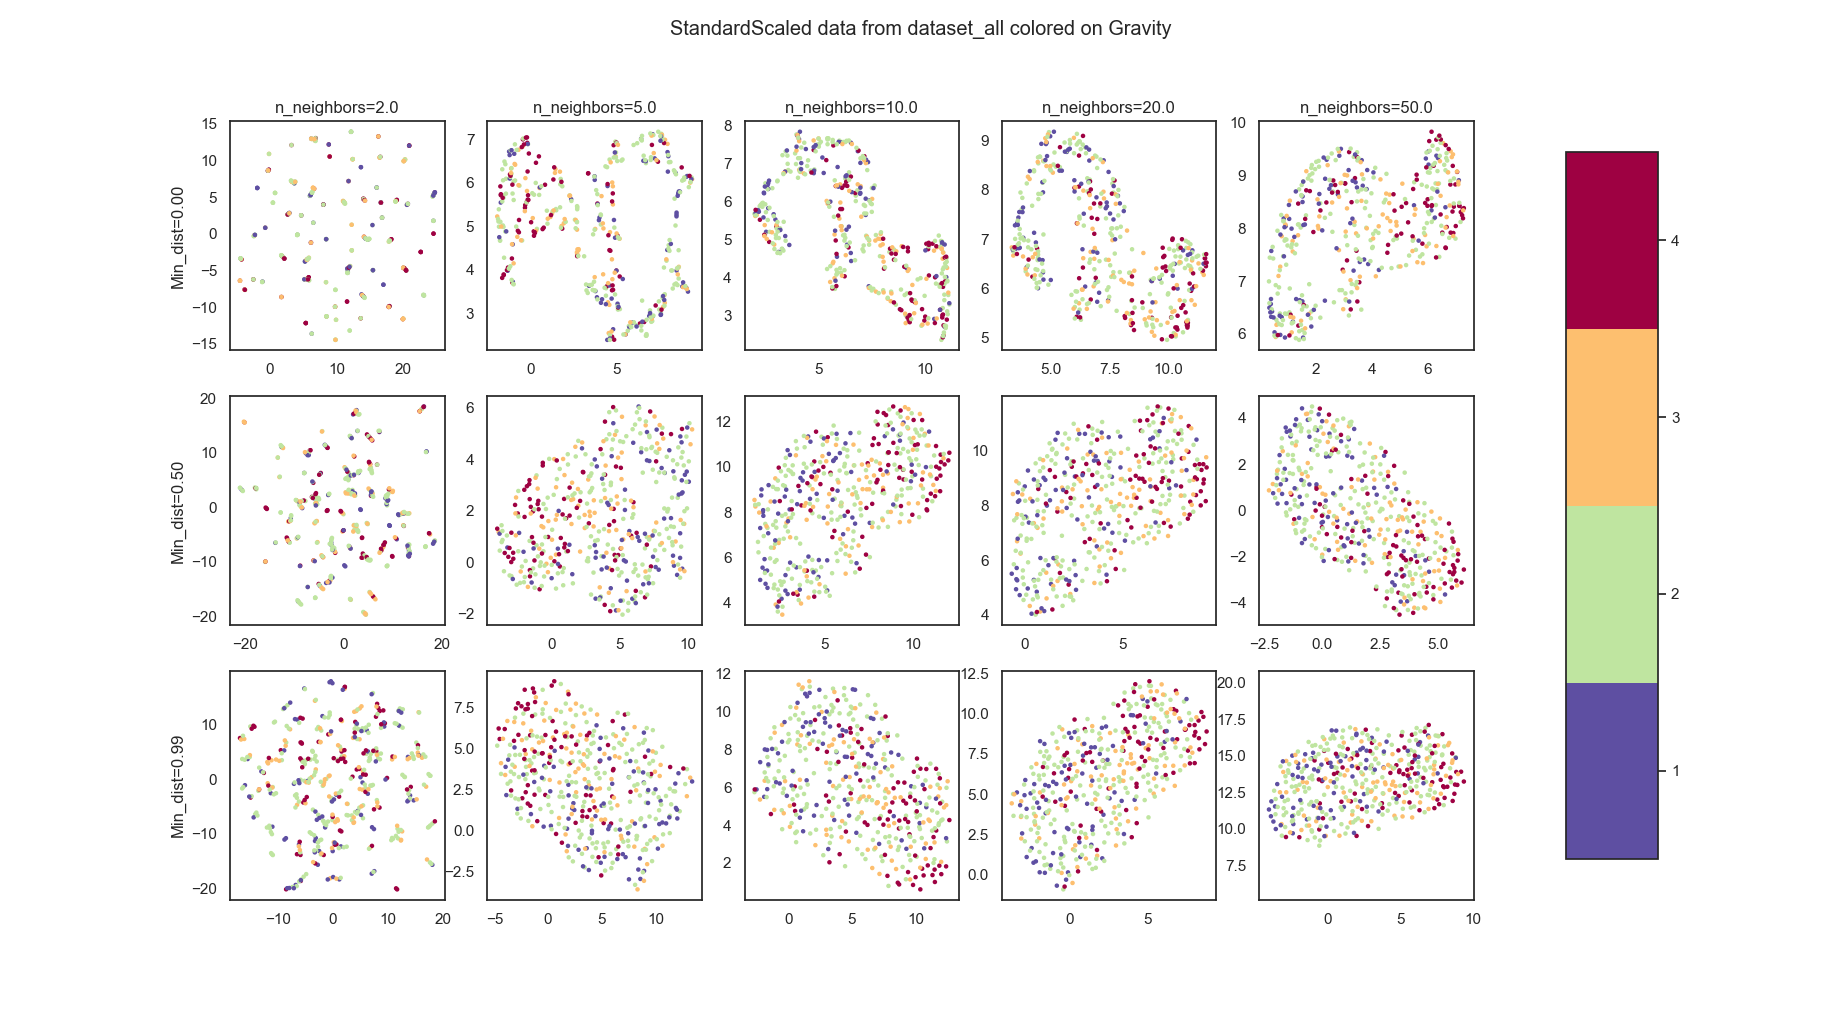
\includegraphics[width = \linewidth]{Scale_umap_gravityquantilies2575.png}
        \caption{Possible combination for umap hyperparameters "number of neighbours" and "minimum distance". Color coding is done with aforementioned gravity score and all the features, i.e. clinical radiomic and radiological, were used.  \label{fig:hyperparam_umap}}
\end{figure}


Also, before proceding, the hyperparameter space for umap was explored since it's the method that allows the most control over rather intuitive parameters.
Changing the value of the minimum distance of points in the final space from 0 to 0.99 changes how the structure is projected, while changing the number of neighbours changes how much the local or global structure of the data influences the final projection.
 Some of the combinations of these parameters can be seen in Figure \ref{fig:hyperparam_umap}


\subsection{PCA}

Starting from PCA, the data was reduced to either two or three dimensions considering clinical and radiomic features, both separated and together.
In this first example there seems to be a kind of left leaning polarization of the dead individuals, however there are no clear separations in the data.

\begin{figure}[h!]
\centering
  		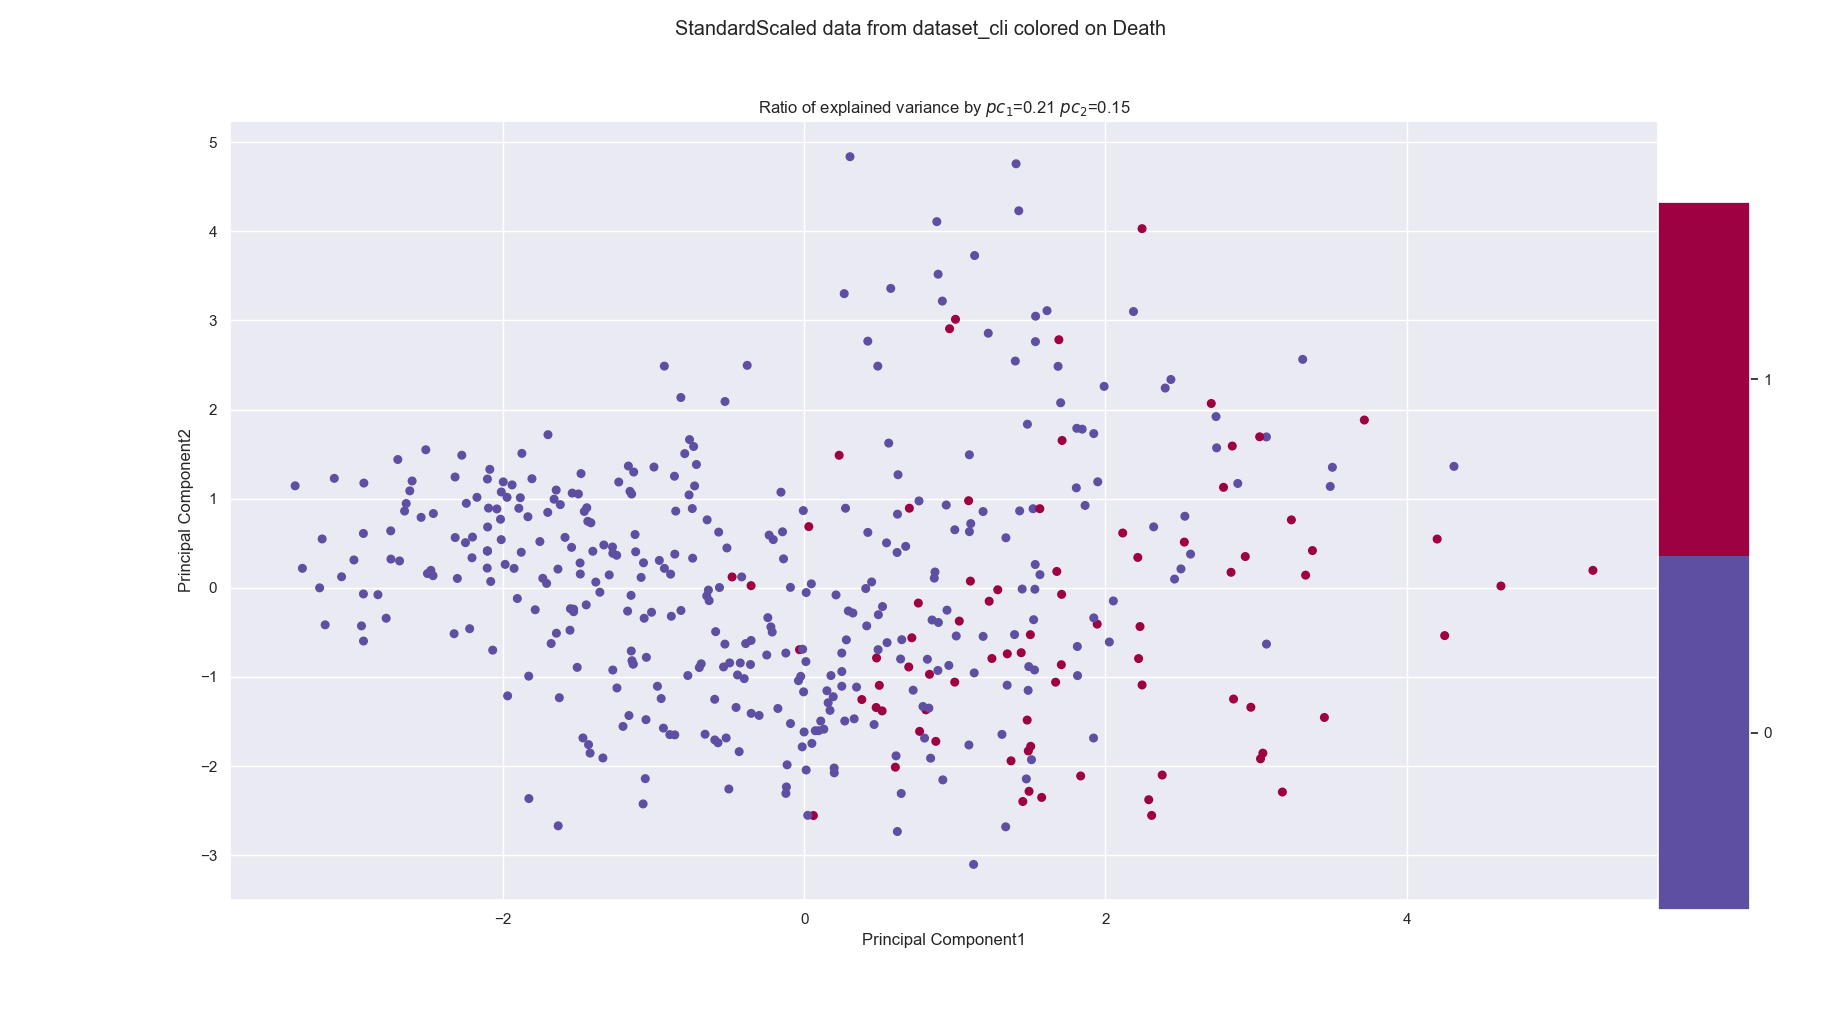
\includegraphics[width=\linewidth]{PCA2_Death.png}
        \caption{2-Principal Component on clinical features.  \label{fig:PCA2_death}}
\end{figure}

 Working on the clinical dataset it can also be noted that the first two components of the PCA explain only 36$\%$ of the total variance. This leads to the conclusion that changes in the data cannot be explained by a single, nor a few, features or linear combination thereof. The next approach was  using the first three principal components using various labels available, most relevant of which being ICU admission, Death and Gravity score.

\begin{figure}[h!]
  		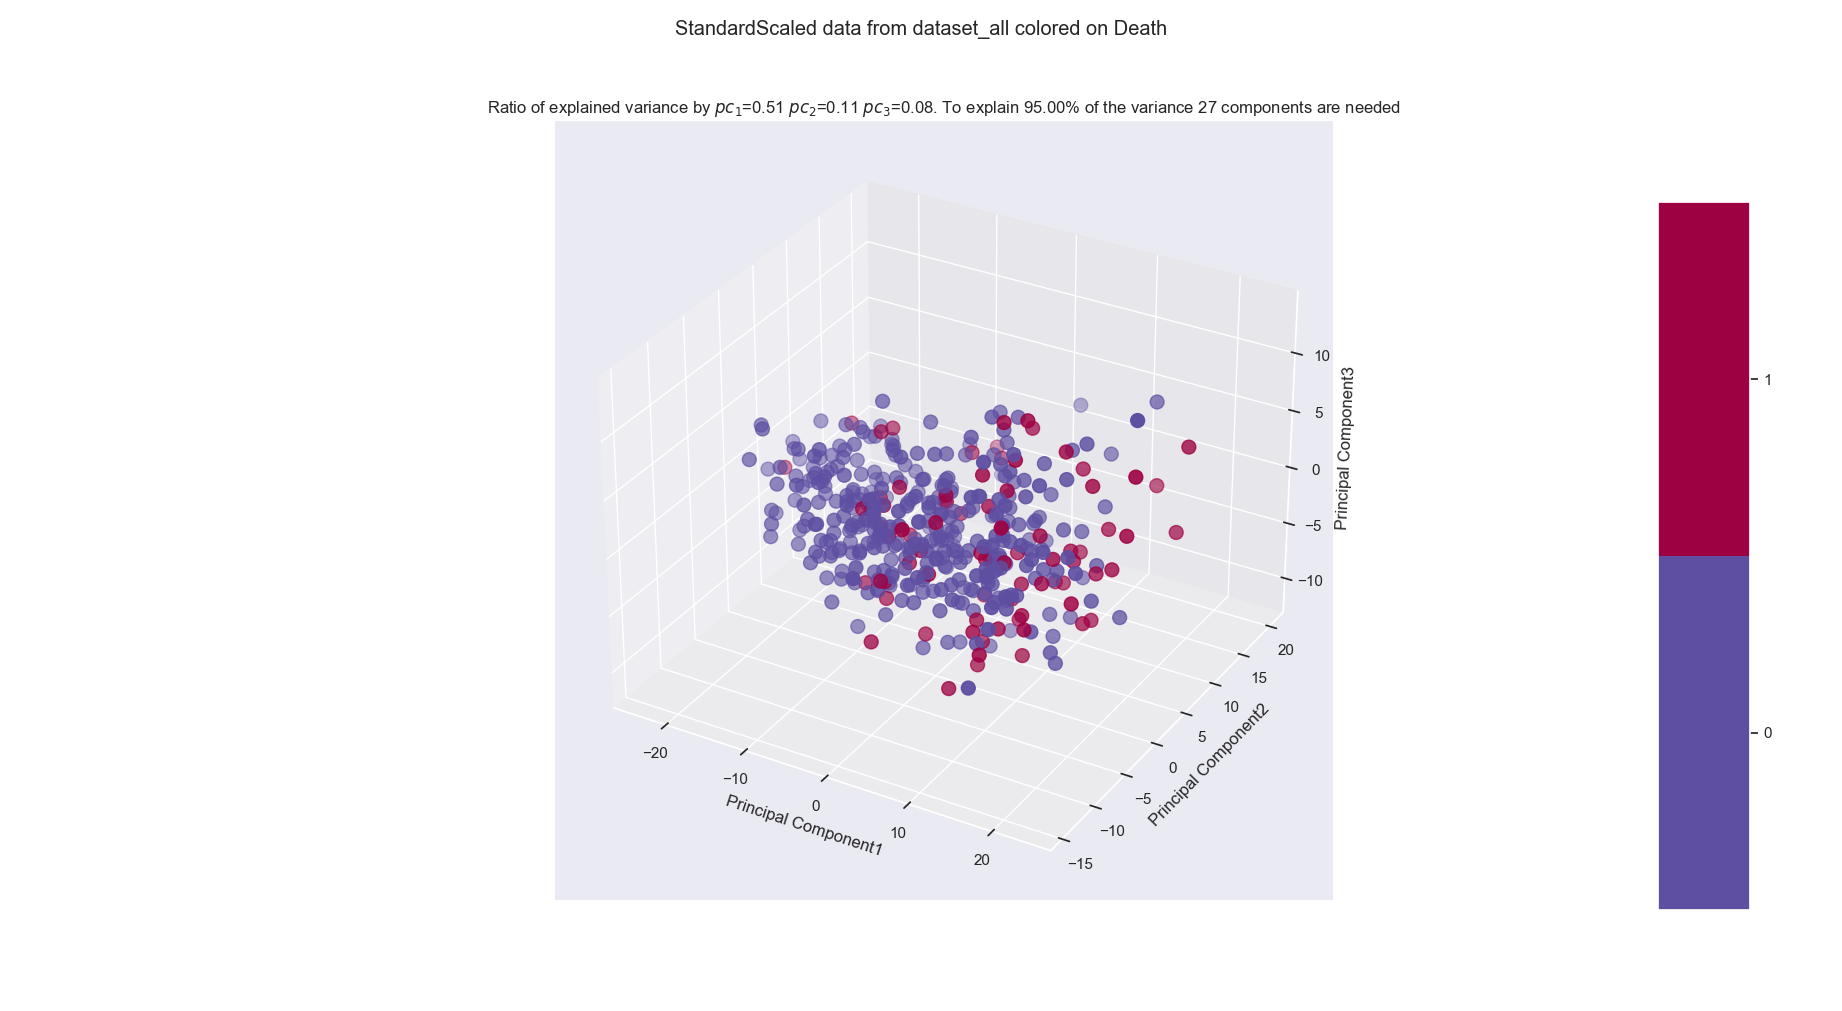
\includegraphics[width=\textwidth]{PCA3_all_Death.png}\label{PCA3_all_death}
  		\caption{3D PCA of whole dataset, colored with death label}
\end{figure}

\begin{figure}[h!]
  		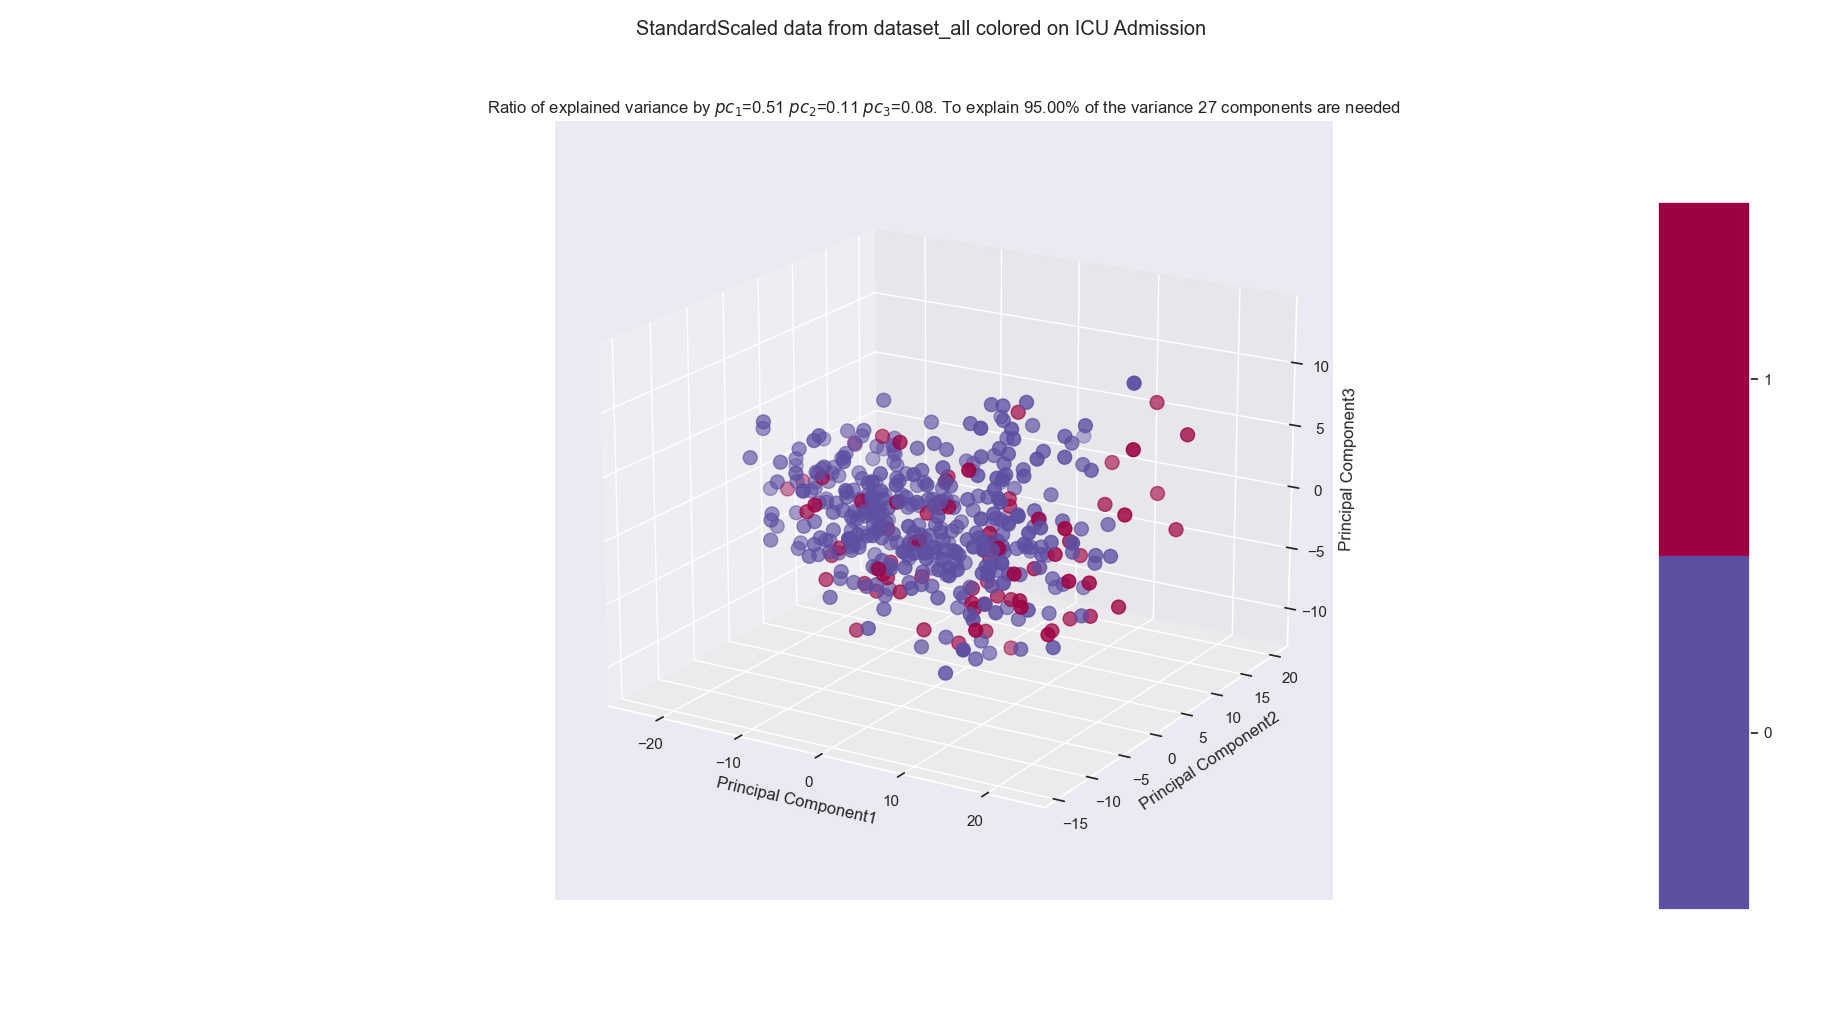
\includegraphics[width=\textwidth]{PCA3_all_ICU.png}\label{PCA3_all_ICU}
  		\caption{3D PCA of whole dataset, colored with ICU Admission label}
\end{figure}

In all cases it seems like introducing the radiomic features causes the loss of the polarization structure that could be seen in the PCA on the clinical dataset alone in fig\ref{fig:PCA2_death}.
 
\begin{figure}[h!]
  		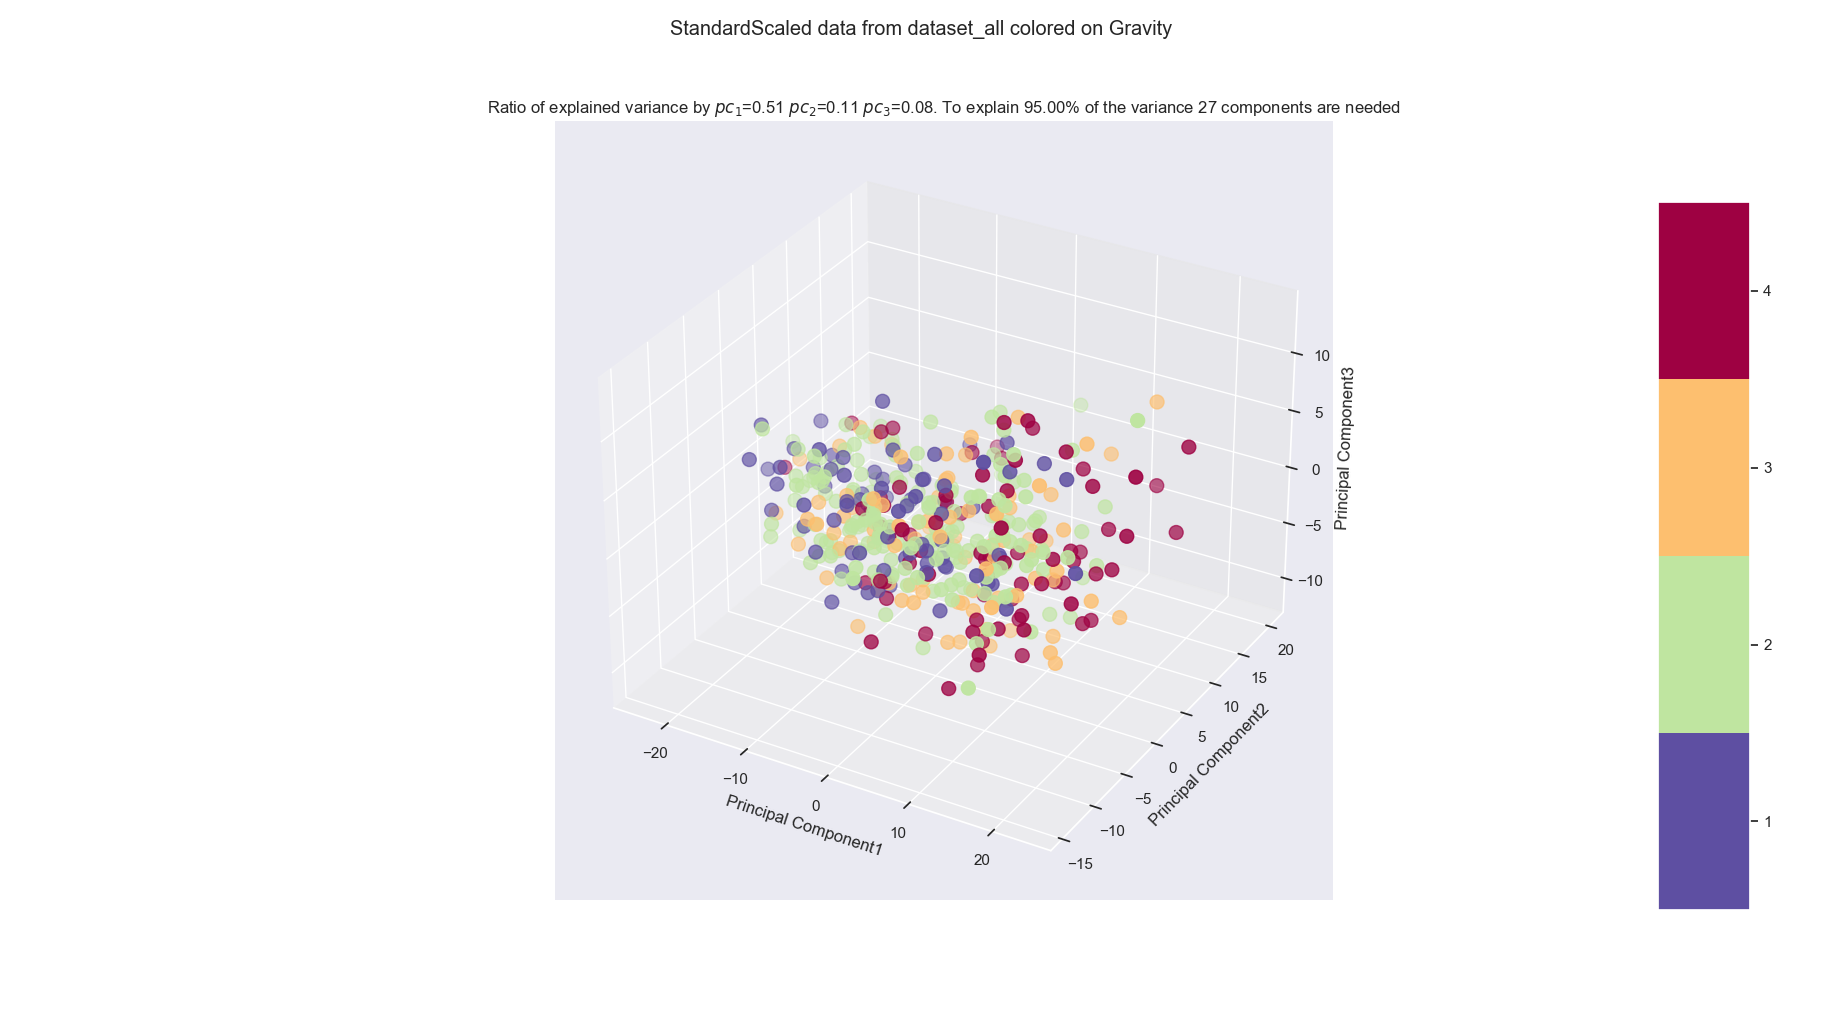
\includegraphics[width=\textwidth]{PCA3_all_Gravity.png}\label{PCA3_all_gravity}
          \caption{Comparison between various colour labels of the top 3 principal components for the entire dataset. Note that to explain 95$\%$ of the variance 27 components would be needed}
\end{figure}

Since there are no visible clusters proceeding with cluster analysis would mean incurring in the risk of finding non meaningful results so it seemed appropriate to try other dimensionality reduction techniques.

The next technique tried was unsupervised Umap. Following the conclusions derived from fig:\ref{fig:hyperparam_umap} the number of neighbours was set to 10 and the minimum distance was set to 0.
Once again the comparison were made between clinical and radiomic dataset as well as different possible labellings. 
Starting from the clinical dataset, without reporting all labels used, it's clear to see that the dataset seems to indicate very local well separated structures which don't seem correlated to gravity outcome

\begin{figure}[htbp]
  		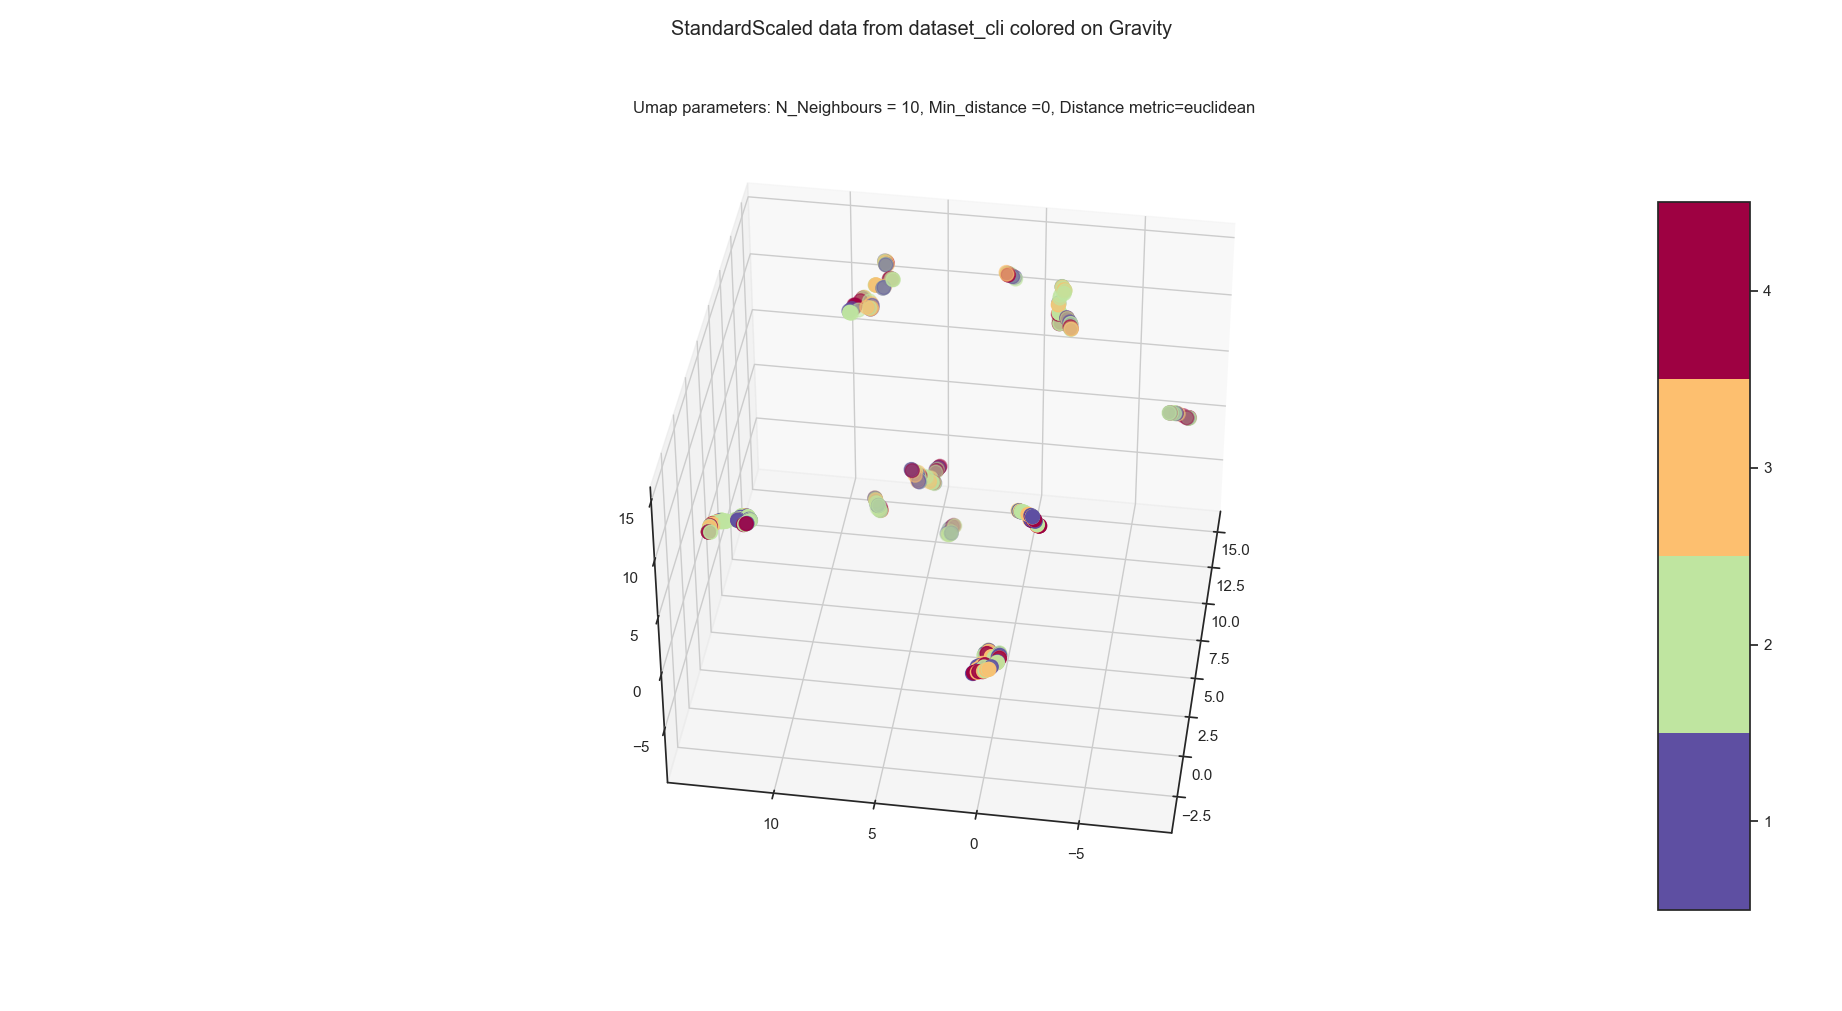
\includegraphics[width=\textwidth]{umap3_cli_Gravity.png}\label{umap3_cli_gravity}
          \caption{3D umap of clinical dataset, colored based on gravity}
\end{figure}

There are 9 well defined groups which don't seem to be correlated to any of the available labels. 
The dimension of these group is also very prohibitive if thinking of further analyses since groups of 35-50 people in a dataset with 15$\%$ mortality rate would mostly be very unbalanced if they were to be used for classification.
However if the introduction of radiomic features were to unite some of these groups then this embedding could be meaningfully used for analysis. 
Looking at the 3D embedding for the whole dataset, the results are:

\begin{figure}[htbp]
  		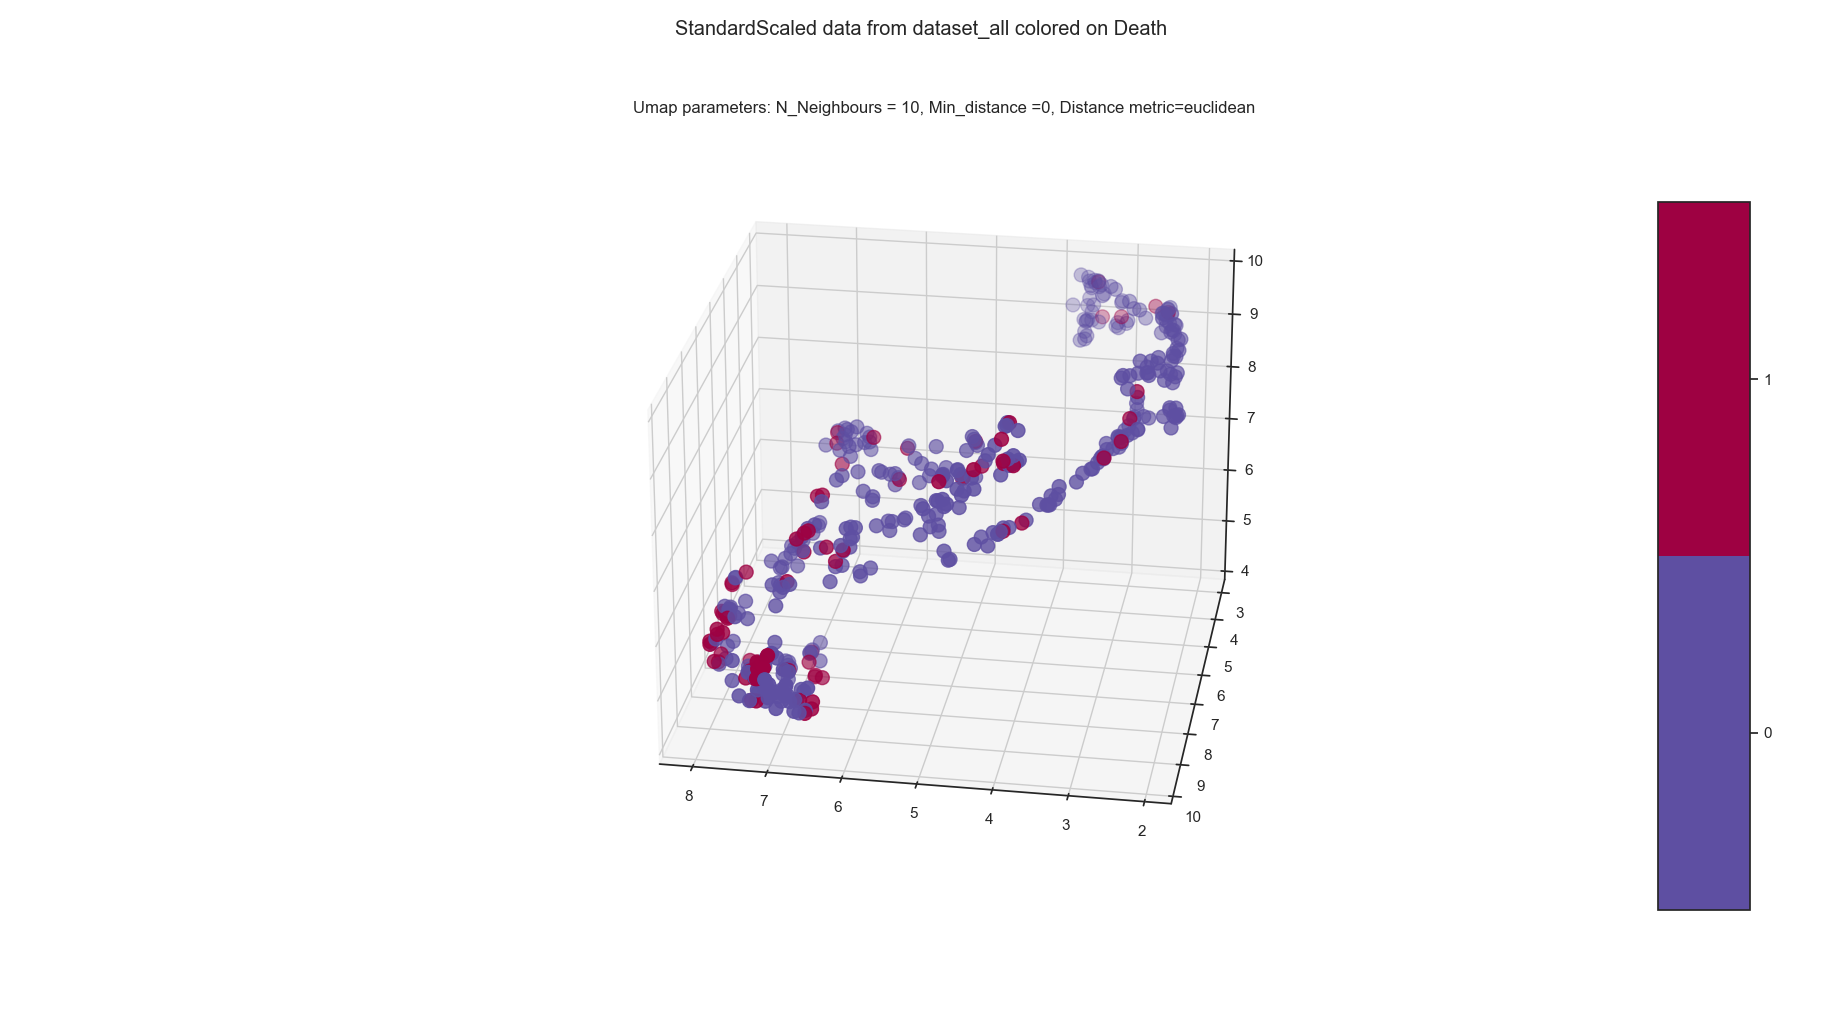
\includegraphics[width=\textwidth]{umap3_all_death.png}\label{umap3_all_death}
          \caption{3D umap of whole dataset, colored based on death}
\end{figure}

\begin{figure}[htbp]
  		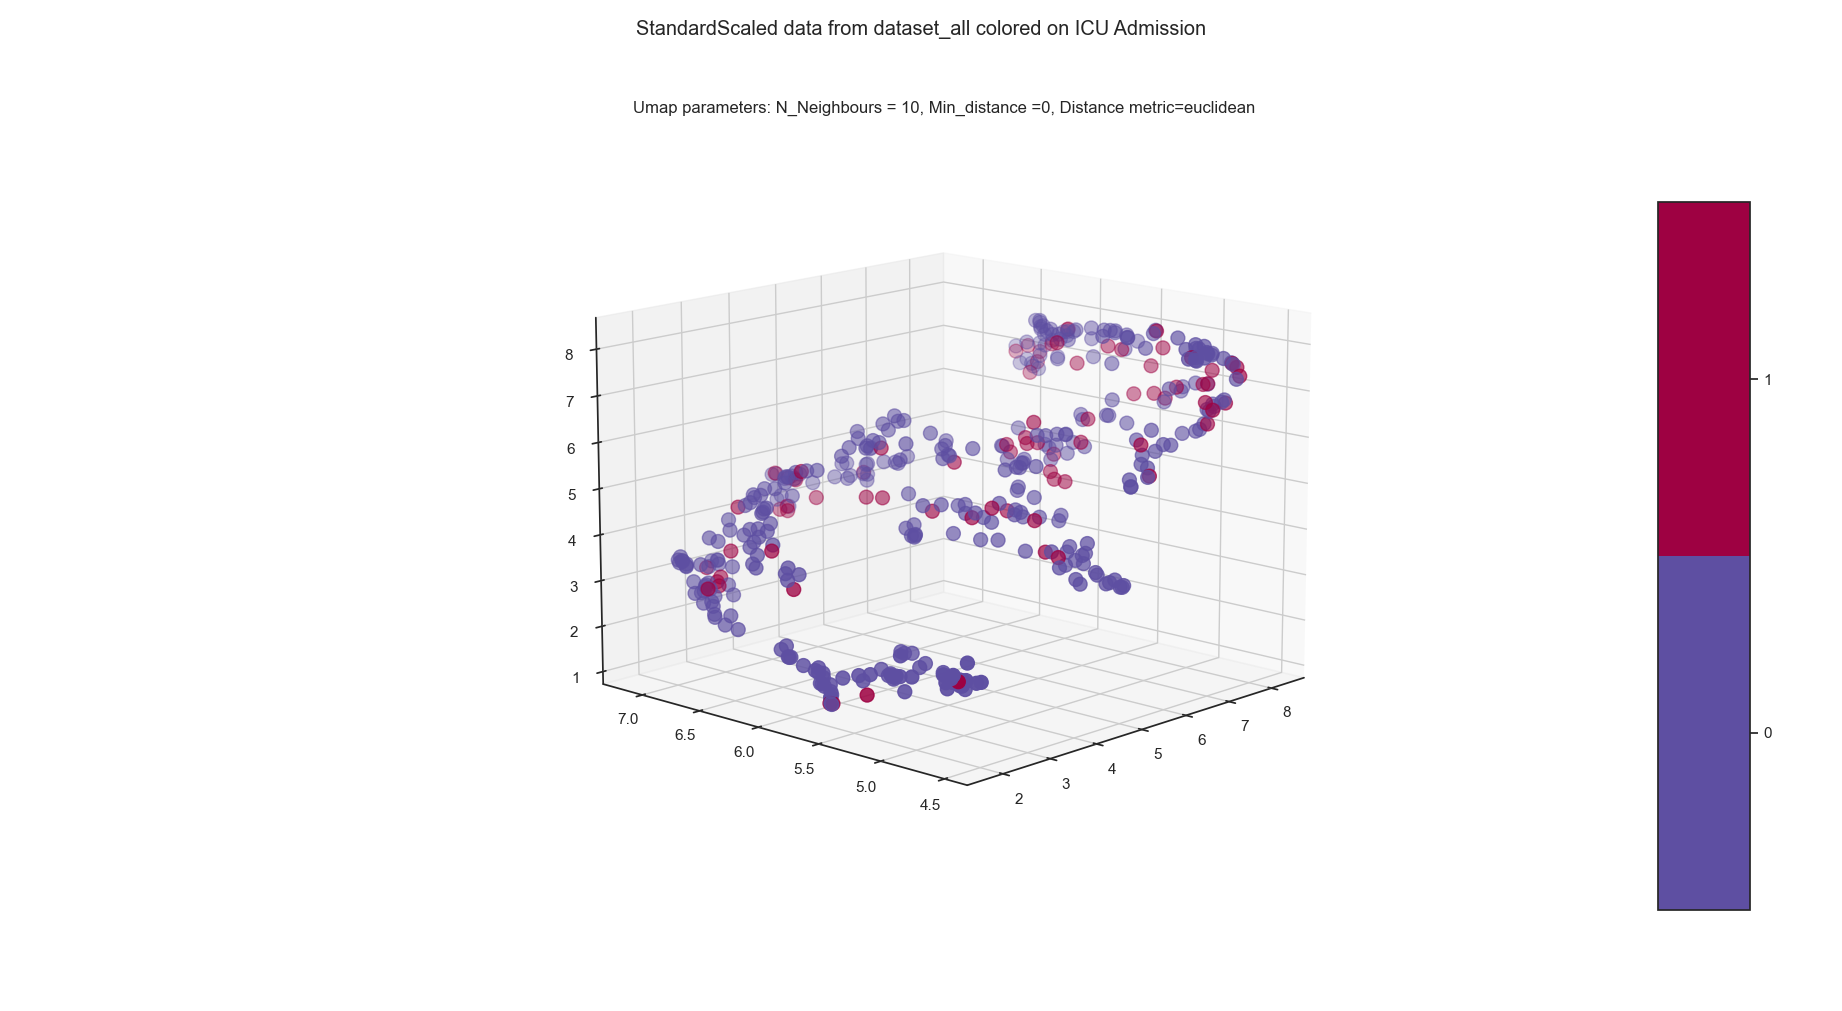
\includegraphics[width=\textwidth]{umap3_all_ICU.png}\label{umap3_all_ICU}
          \caption{3D umap of whole dataset, colored based on ICU admission}
\end{figure}

\begin{figure}[htbp]
  		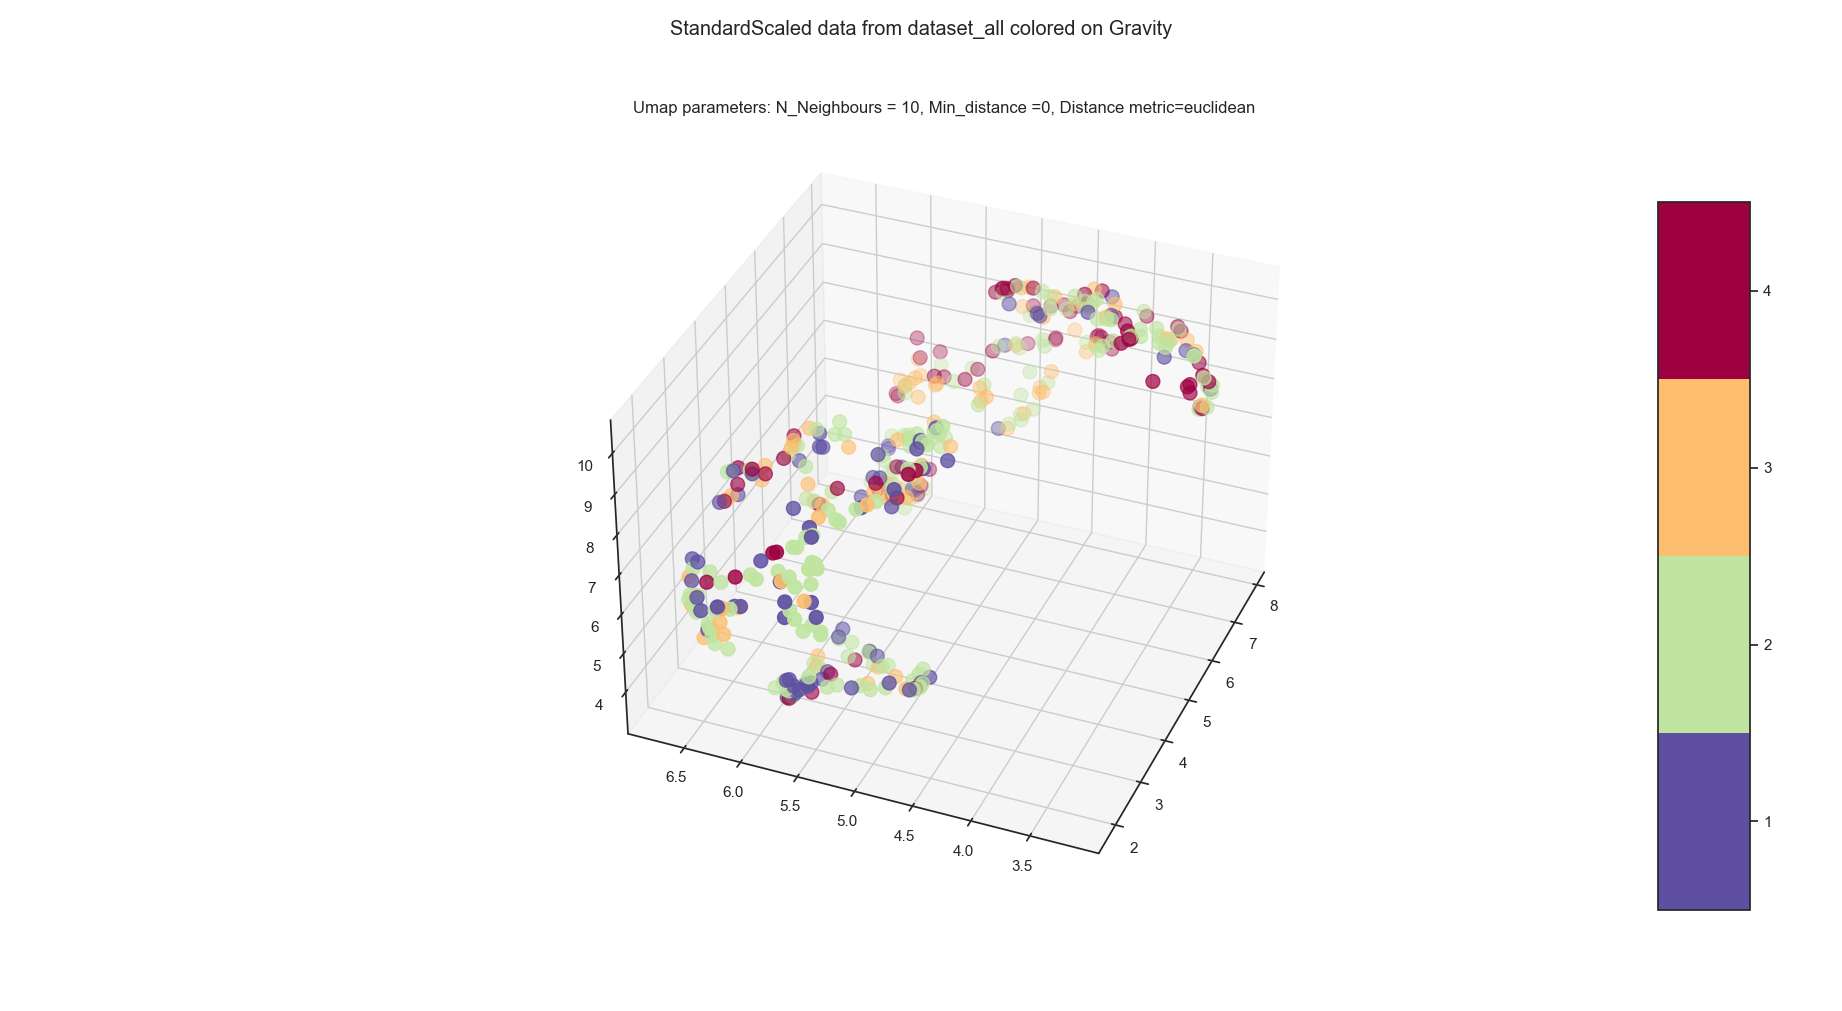
\includegraphics[width=\textwidth]{umap3_all_Gravity.png}\label{umap3_all_Gravity}
          \caption{3D umap of whole dataset, colored based on gravity}
\end{figure}

Once again the introduction of the radiomic feature seems to be a confounding factor in the seemingly clear-cut order present in the clinical dataset alone.
There seems to be a well connected structure, which makes sense because umap sets out with the objective of preserving said structure.
However since the variables of interest as label are Death, ICU admission or some kind of combination of them with hospital permanence there seems to be no visual correlation between structure and label.
As such the next dimensionality reduction was tried to see if it yielded better results.
 
Moving on from unsupervised methods to a supervised one, PLS-DA was used giving as label both death and ICU using both whole dataset, and singularly radiomic or clinical features. 
Starting from the clinical features alone, predicting on death Figure~\ref{PLSDA-Clinical} can be obtained.

\begin{figure*}[htbp]
  		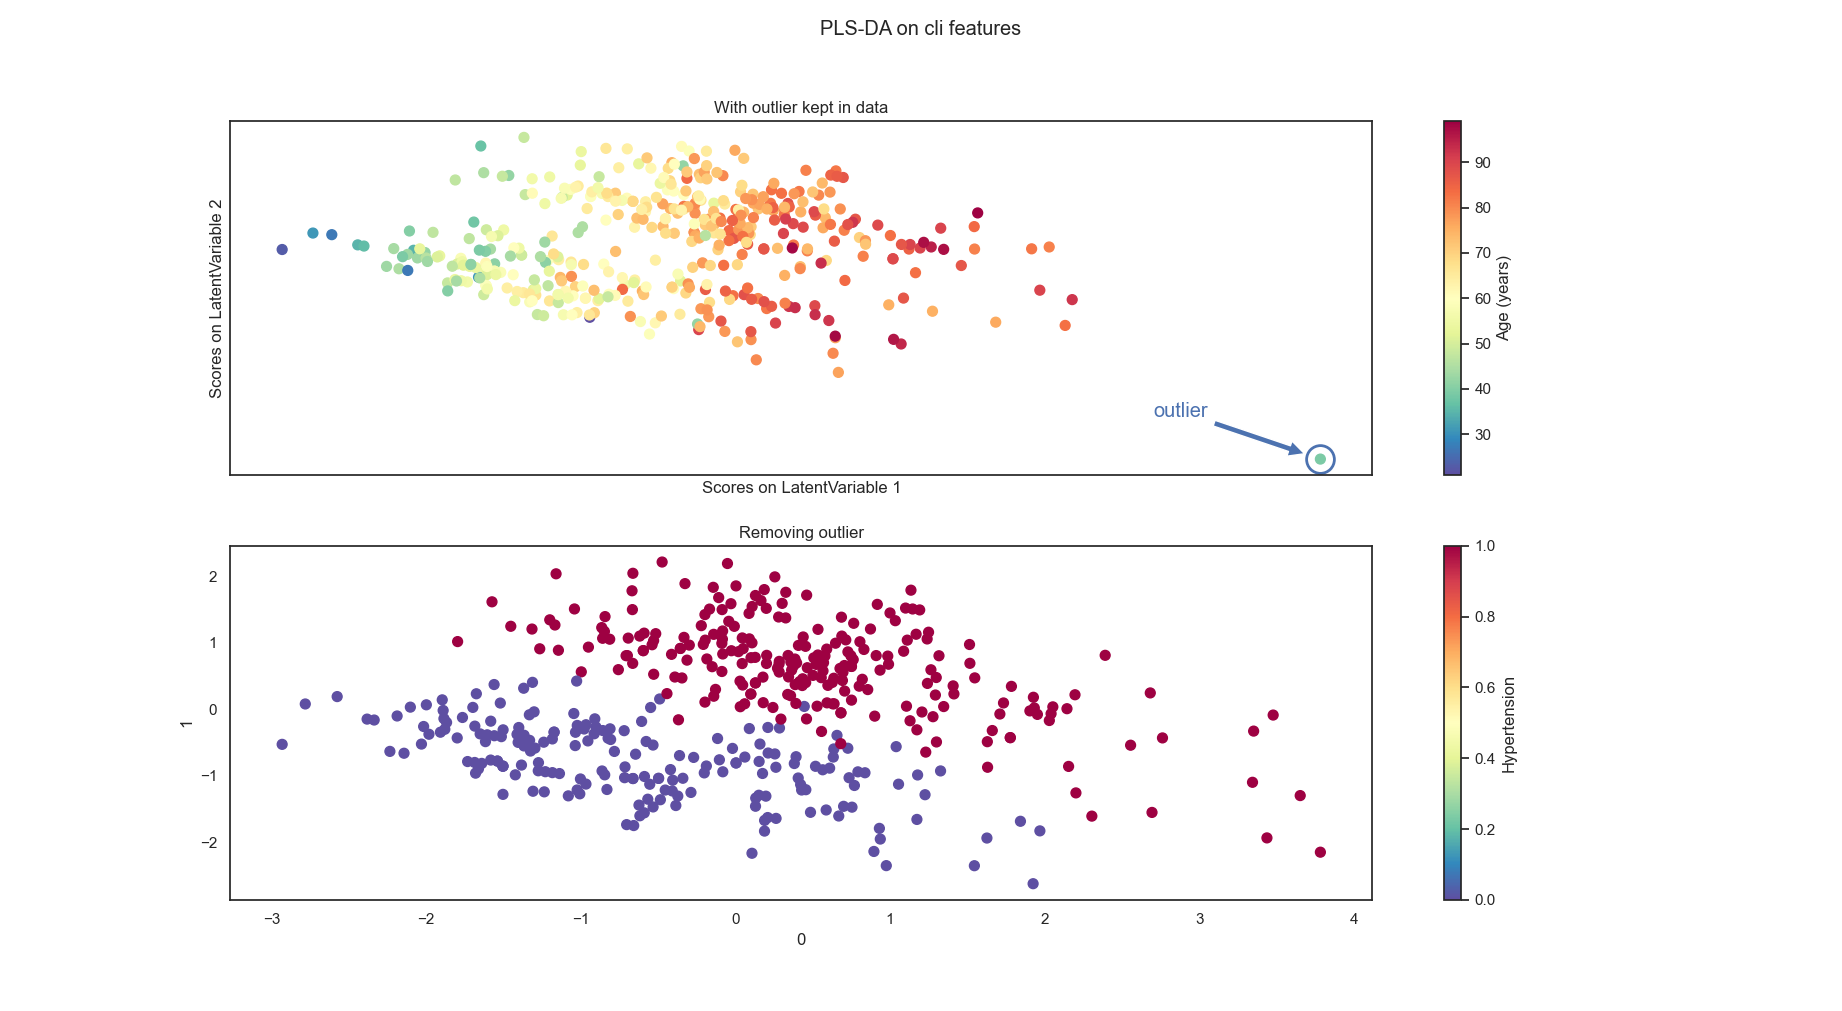
\includegraphics[width=1\textwidth]{Clinical_dataset.png}
          \caption{PLS-DA predicting on death coloured with age and hypertension\label{PLSDA-Clinical}}
\end{figure*}

In Figure~\ref{PLSDA-Clinical} there are a few things to note. 
The first is the presence, in the top plot, of an outlier which, since PLS-DA is based on minimization of least squares, can ruin a lot the performance of the procedure. 
For this reason in the second plot the outlier was removed and the algorithm was run again on the cleaned data.
The second thing to notice is the coloring used which, in the first plot, was used to highlight that along the one of the two latent variables the data is roughly distributed depending on age while, in the second plot, was used to highlight that the algorithm is able to perfectly separate the subjects with hypertension from those without it.
However, by looking at the same embedding labelled with death and ICU admission fig \ref{PLSDA-Clinical-death} can be obtained

\begin{figure}[htbp]
  		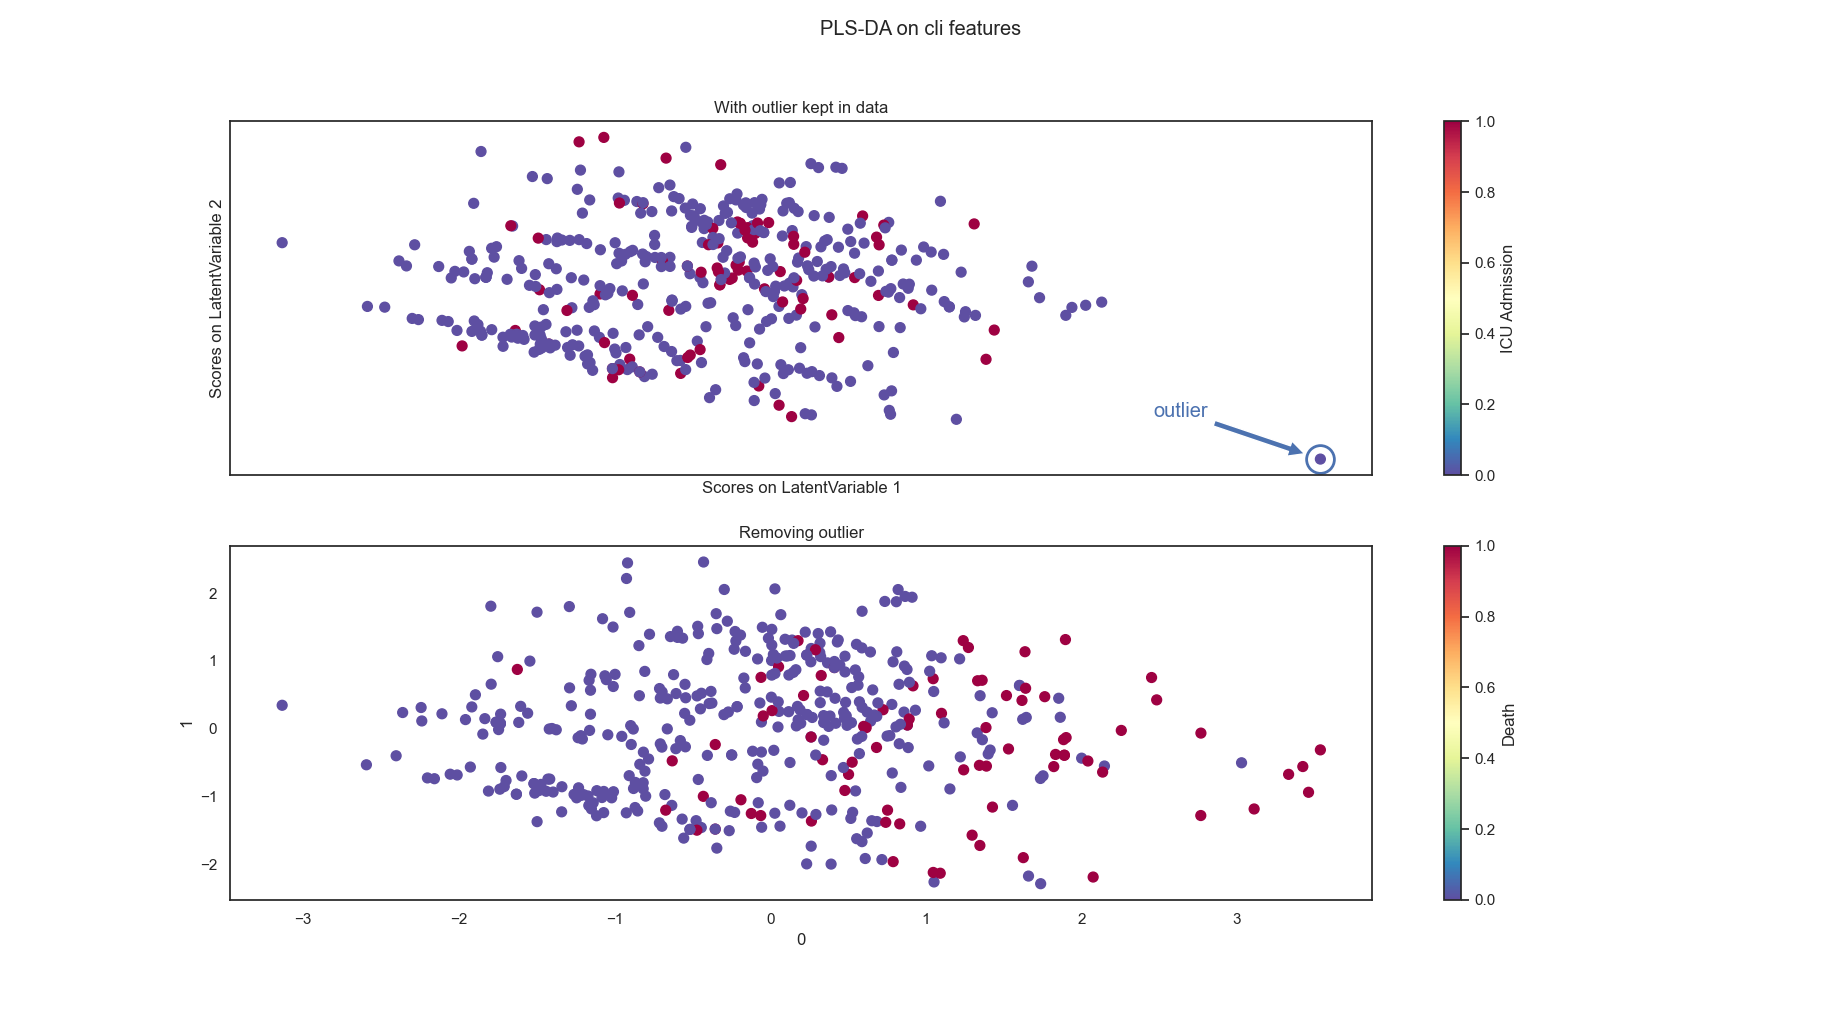
\includegraphics[width=\textwidth]{PLSDA_cli_death.png}
          \caption{PLS-DA predicting on death coloured with death(bottom) and ICU Admission(top)\label{PLSDA-Clinical-death}}
\end{figure}

It's clear to see that, when predicting on death, the PLS-DA algorithm doesn't find any behaviour relevant for ICU admission.
It's also clear that there is at least a pattern of points labeled as dead being towards the right of the image, this can be easily explained by looking at how the ages are distributed in the first plot of fig: \ref{PLSDA-Clinical}. 
From this it's possible to deduce that older individuals tend to die more and that hypertension does not seem to be relevant when considering death as a clinical outcome.
If necessary the PLS-DA algorithm allows also to see the weights given to the features in predicting the label. At least for the clinical dataset, which has a reasonable number of features, it's interesting to report it ordering the coefficients by descending absolute value: 

\begin{table}
\caption{PLS-DA feature weights in prediction on death using clinical features}
\centering
	\begin{tabular}{|l|r|}
	\hline
	Feature Name &         Importance \\
	\hline
	 Respiratory Rate &  0.120206 \\
	 Age (years) &  0.116305 \\
	 Obesity &  0.004293 \\
	 Hypertension & -0.004626 \\
	 History of smoking & -0.012314 \\
	 Febbre & -0.045431 \\
	 Sex\_bin & -0.054947 \\
	\hline
	\end{tabular}
\end{table}

Doing the exact same procedure on the whole dataset, which means by including the radiomic features, Figure~\ref{fig:whole_dataset} can be obtained.

\begin{figure}[htbp]
  		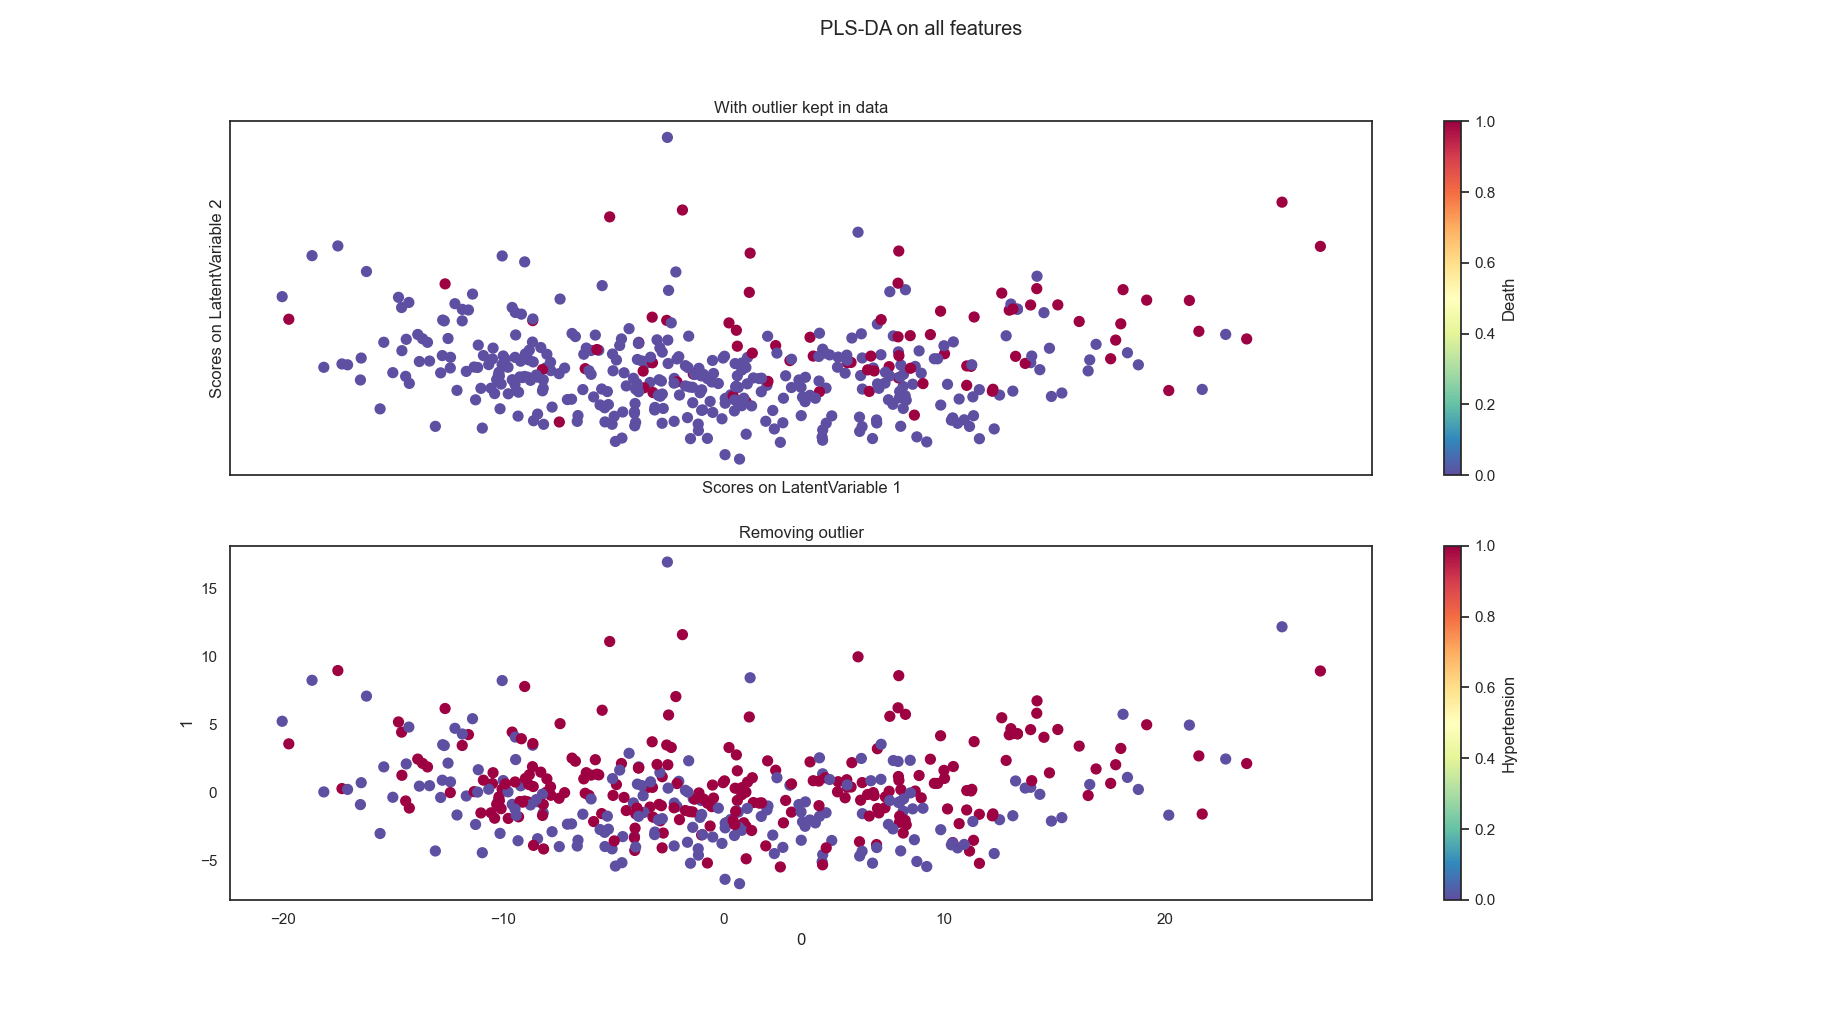
\includegraphics[width=\textwidth]{Whole_dataset.png}
          \caption{PLS-DA predicting on death coloured with death(top) and hypertension(bottom) on whole dataset\label{fig:whole_dataset}}
\end{figure}



\begin{figure*}[htbp]
  		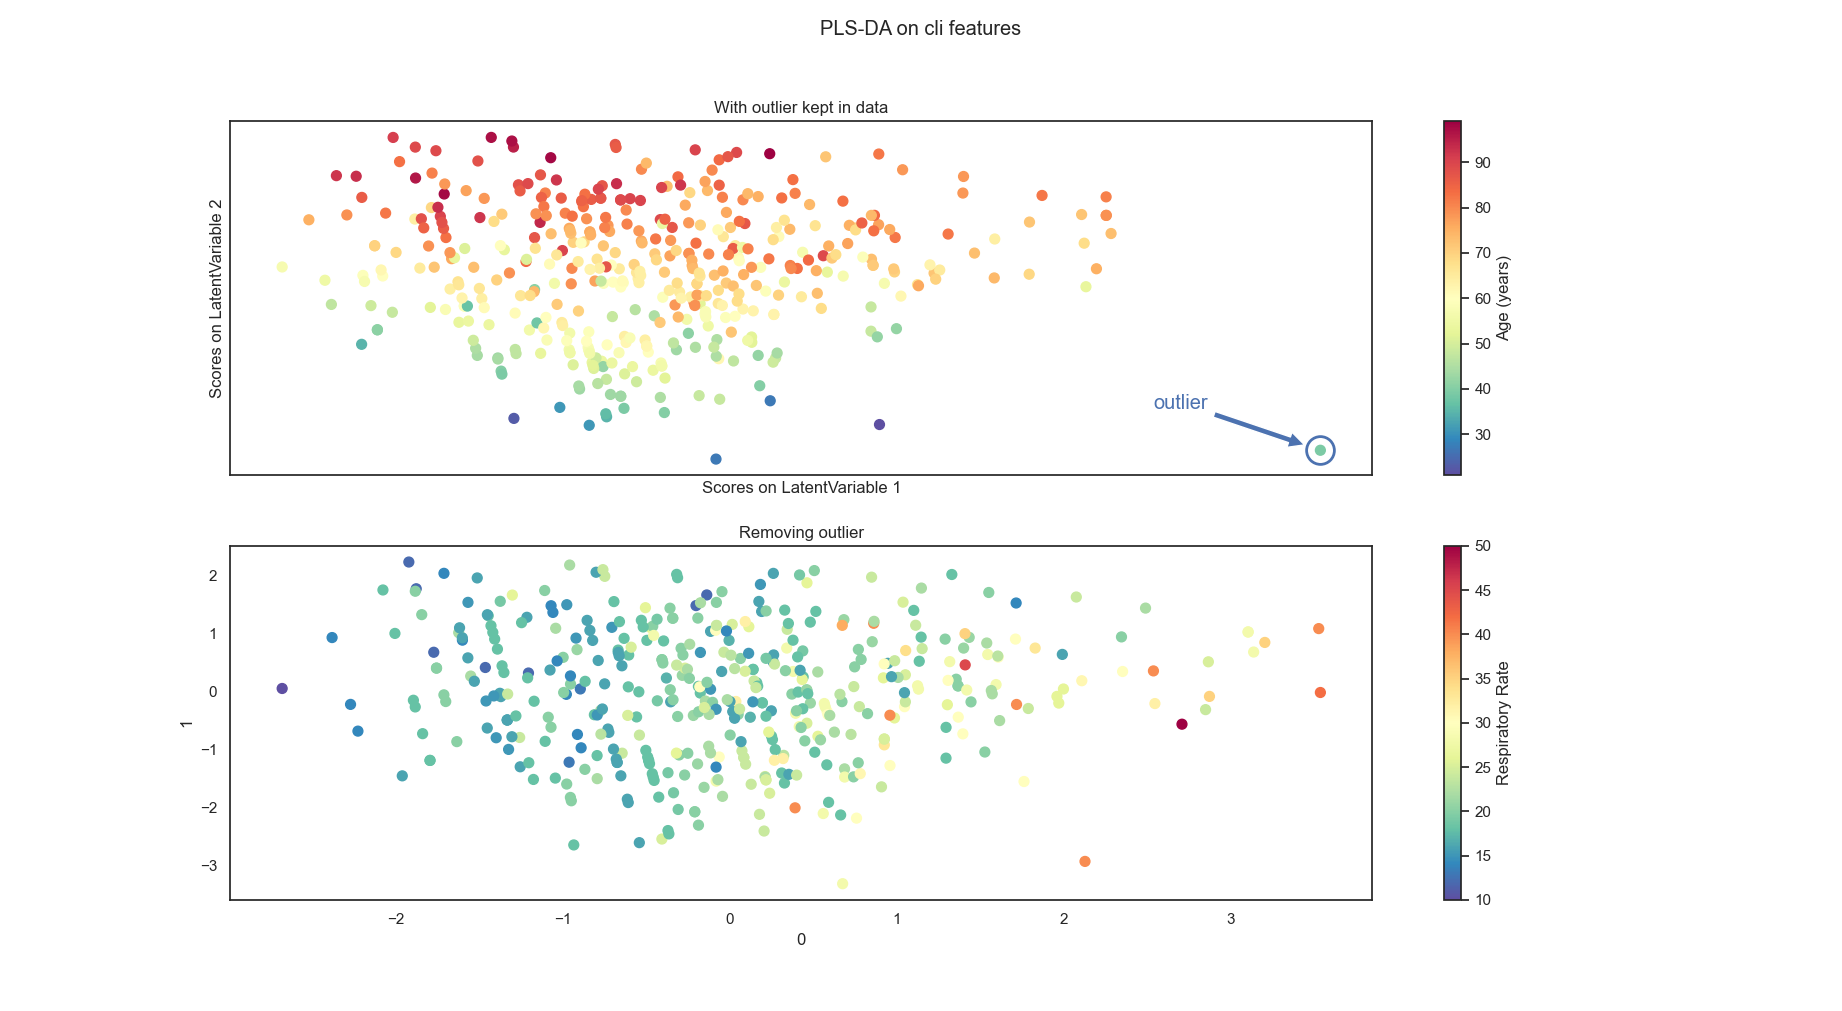
\includegraphics[width=1\textwidth]{PLSDA_cli_ICU_LV.png}
          \caption{PLS-DA predicting on death coloured with Age and respiratory rate on clinical features\label{fig:PLSDA-ICU-LV}}
\end{figure*}

Once again adding the radiomic features has evidently introduced noise in the system, which no longer displays any kind of behaviour, pattern nor separation.
Doing the same analysis but using ICU Admission as a label Figure~\ref{fig:PLSDA-ICU-LV} can be obtained. 

Now the colors have been chosen to highlight that respiratory rate and age have the main role in determining the latent variables. However, in this case, there doesn't appear to be a clear cut distinction as it happened before with hypertension.
Looking at how the points scatter by coloring them according to the two interesting clinical labels the following figure can be obtained:

\begin{figure}[H]
  		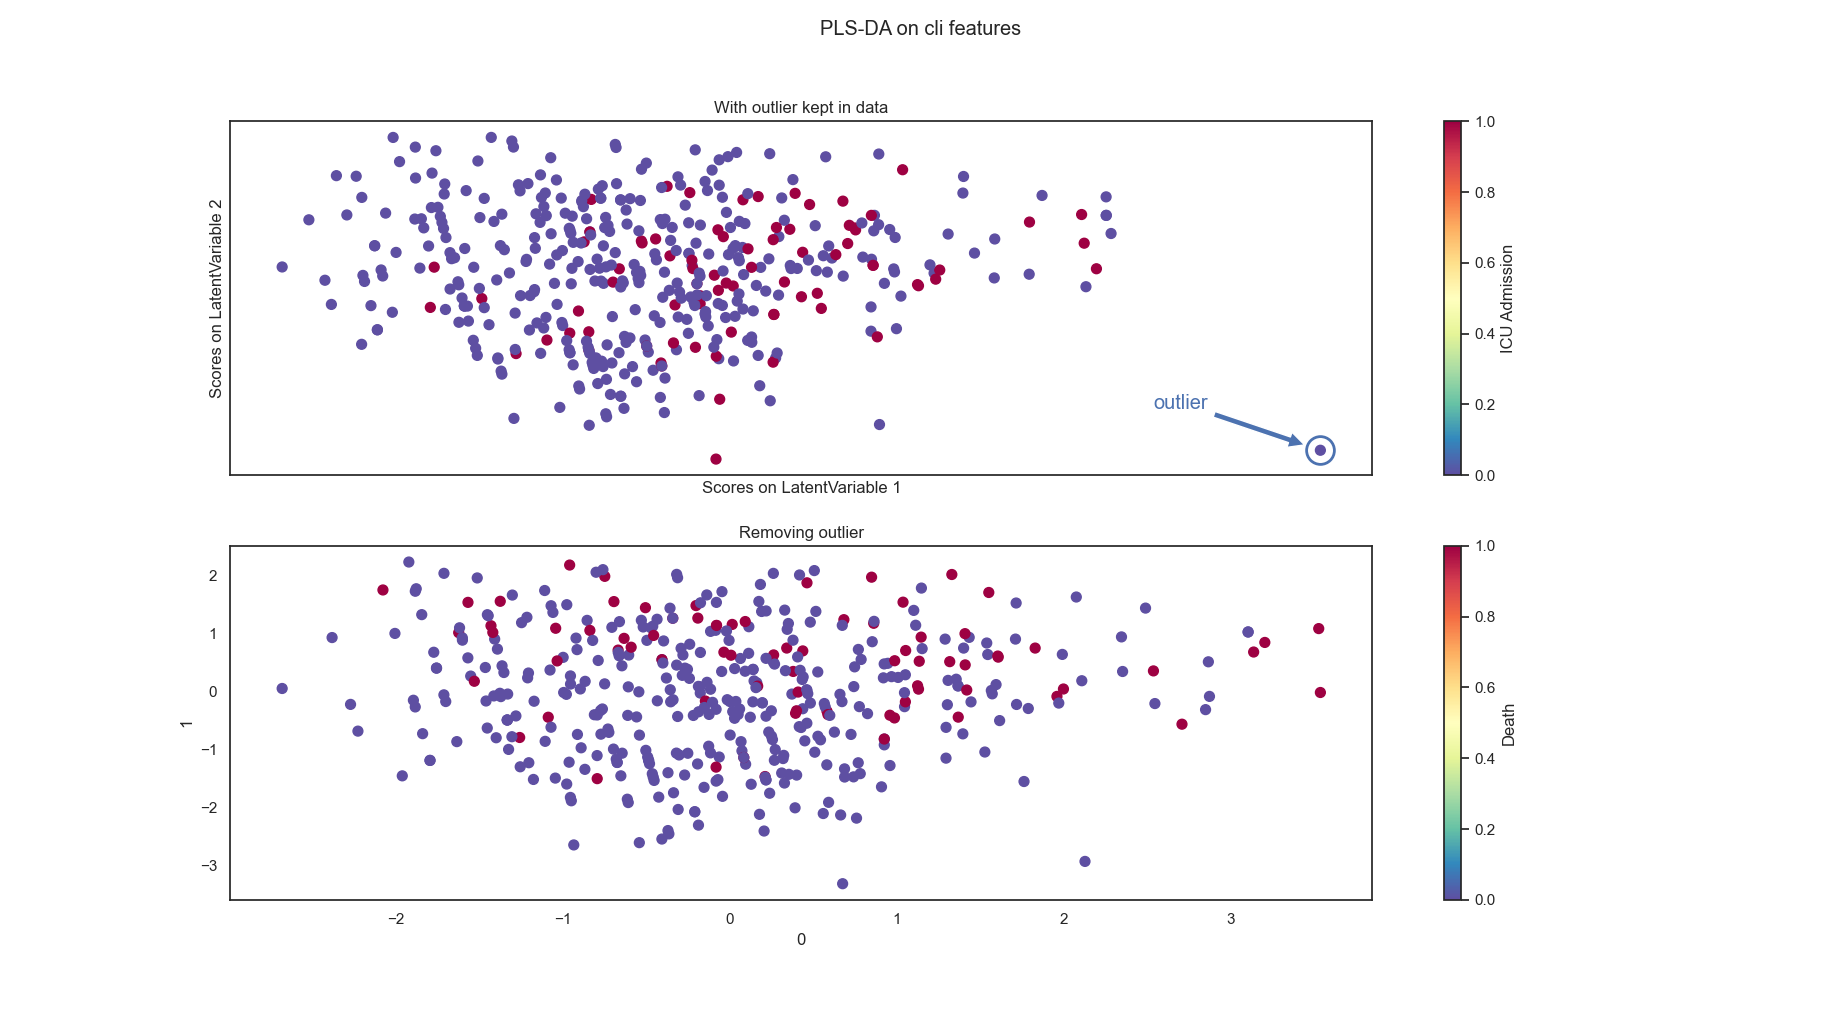
\includegraphics[width=\textwidth]{PLSDA_cli_ICU.png}
          \caption{PLS-DA predicting on death(bottom) coloured with death and ICU admission(top) on clinical features\label{fig:PLSDA-ICU}}
\end{figure}

Finally, introducing the radiomic features in the analysis the usual effect of reducing separation can be seen can be seen in the figure below:

\begin{figure}[H]
  		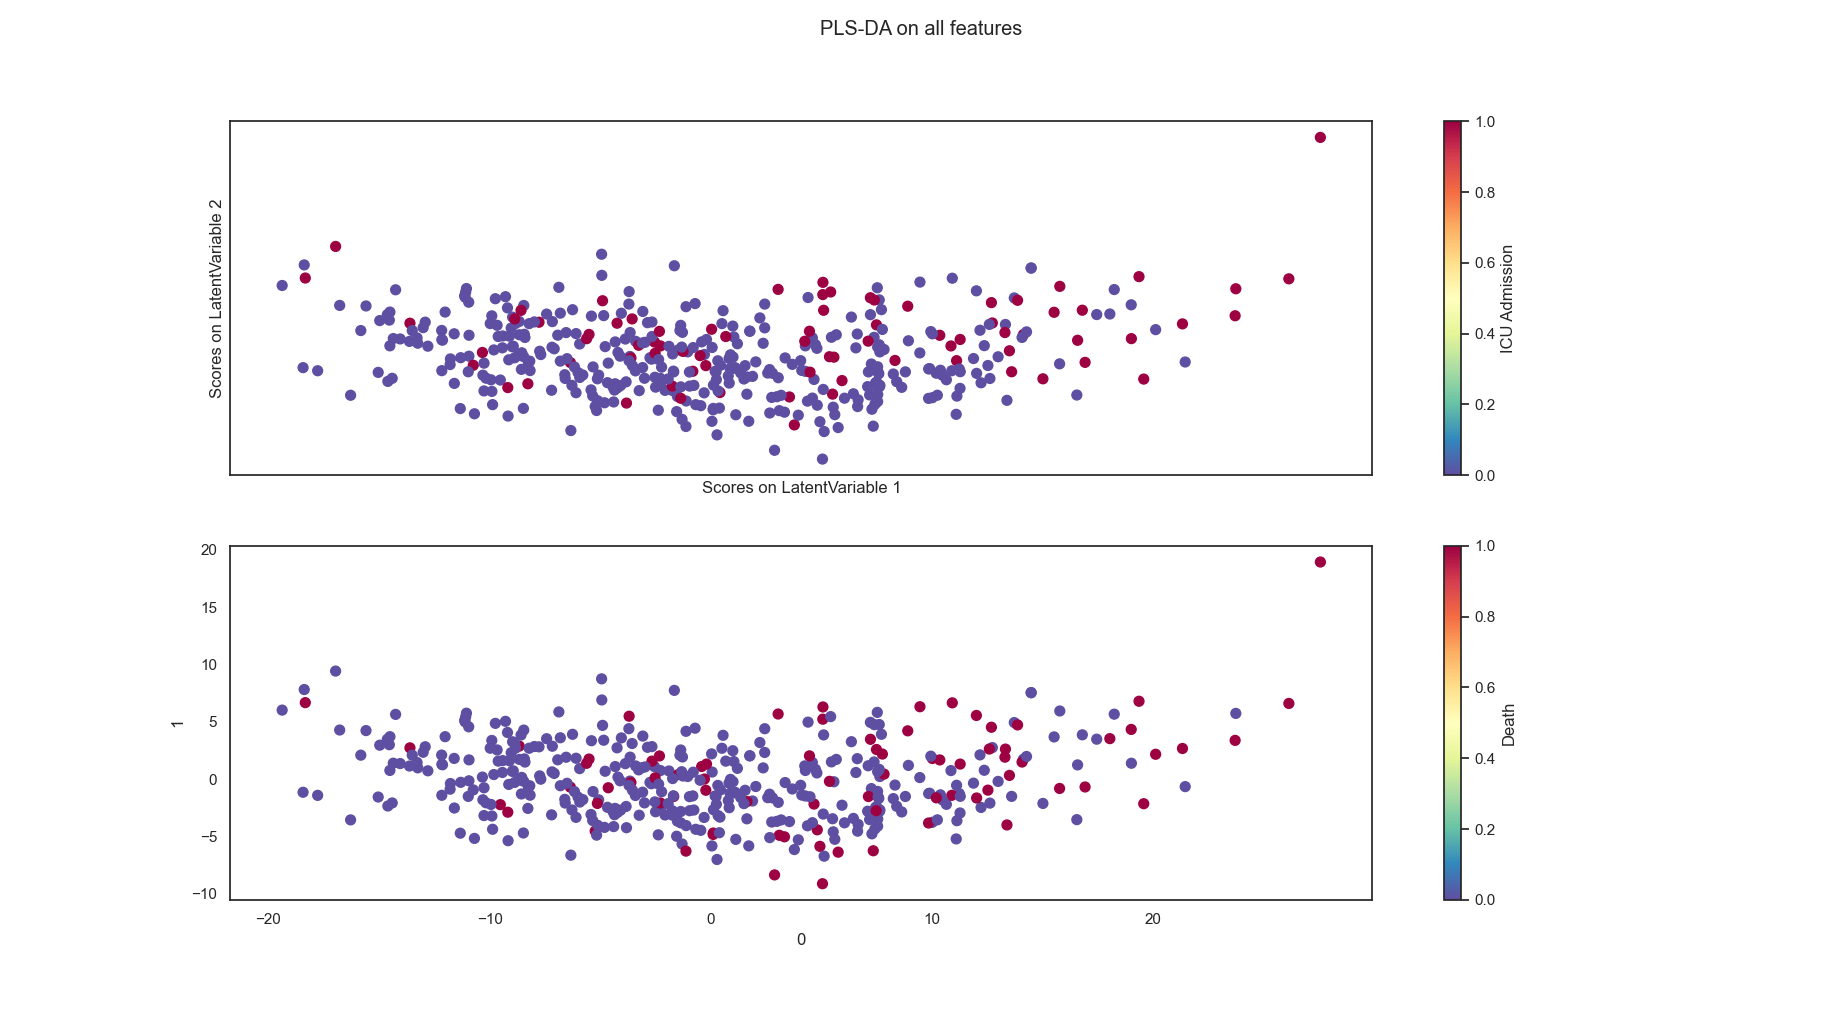
\includegraphics[width=\textwidth]{PLSDA_all_ICU.png}
          \caption{PLS-DA predicting on death coloured with death(bottom) and ICU admission(top) on all available features\label{fig:PLSDA-ICU-all}}
\end{figure}
 